%\documentclass[twocolumn]{article}
\documentclass[./exercises.tex]{subfiles}
\begin{document}

\textit{\textbf{Stellariumlabb  } }

\section{Stjärnor och stjärnbilder}
\begin{itemize}
    \item[--] Är det några av dessa objekt som aldrig kan ses från Stockholm? Varför? Vilka kan alltid ses en
klar natt? Vilka kan ses ibland och när är det?\\
\begin{enumerate}[label=(\alph*)]
\item Andromeda (And) Andromedagalaxen (M31)\\
Verkar alltid vara synlig från Stockholm året runt, åtminstone om man tidstegar i Stellarium.
Observationsplugin säger dock att denna befinner sig nattetid över horisonten fr.o.m. 1 Jan till
15 Maj och därefter fr.o.m. 30 Juli till 31 Dec.

\item Lilla Björn (UMi) Polstjärnan ($\alpha$-UMi)\\
Alltid synlig

\item Stora Björn (UMa) Karlavagnen\\
Alltid synlig
\item  Oxen (Tau) Krabbnebulosan (M1), Sjustjärnorna el. Pleiaderna (M45)
Ej möjligt att se under ca April till Oktober då siktlinjen ligger alldeles för nära solen.
\begin{figure}[H]
\centering
  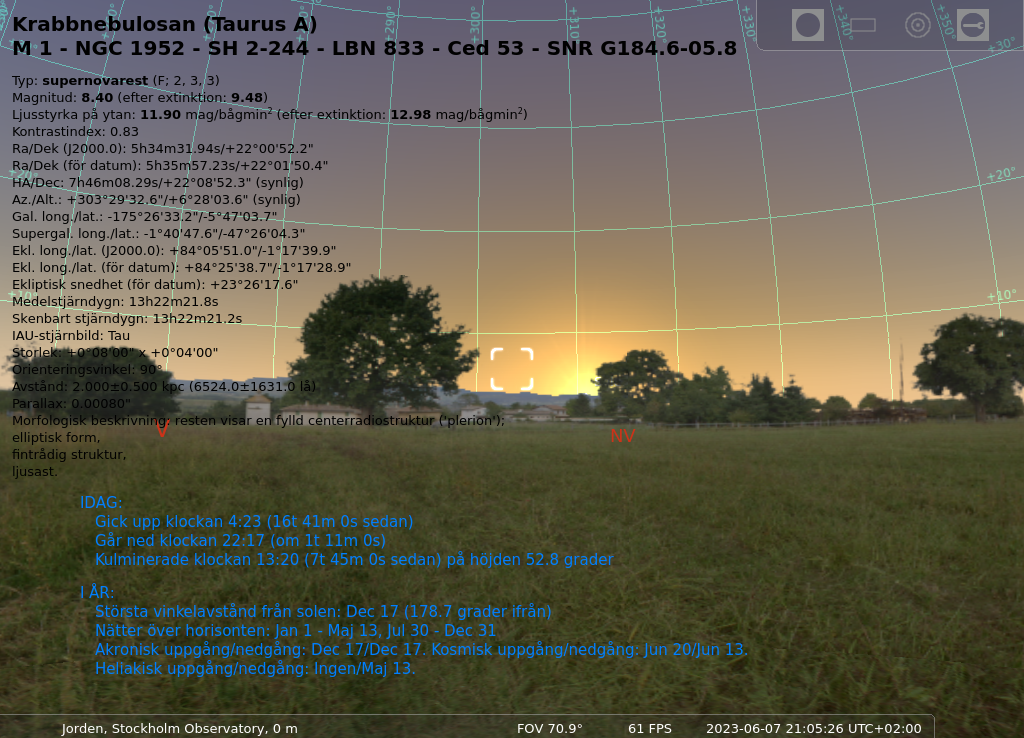
\includegraphics[scale=0.35]{stellarium-001.png}
  \caption{Krabbnebulosan sommartid}
  \label{fig4}
\end{figure}
\item Perseus (Per) Öppen stjärnhop (NGC869, 884)\\
Synlig, dock verkar det inte vara särskilt långa stunder under sommaren som den är observerbar.

\item Herkules (Her) Två klotformiga stjärnhopar (M13, M92)\\
M13 ligger stundtals väldigt nära horisonten. Svårt att avgöra om hela M13 är synlig då man tidsstegar i hög hastighet
med hög utzooming. Observationsappen i Stellarium indikerar dock att varken M13 eller M92 har någon akronisk eller helikalisk
 uppgång/nedgång vilket måste betyda att stjärnhoparna hela tiden är synliga.

\item Lyran (Lyr) Vega och Ringnebulosan (M57)\\
Vega är alltid synlig men Ringnebulosan ser ut att ligga strax under eller på horisontlinjen.
Observationsappen i Stellarium indikerar dock att M57 inte har någon akronisk eller helikalisk
 uppgång/nedgång vilket måste betyda att den är synlig året om.
 
\item Orion (Ori) Orion-nebulosan (M42), Hästhuvudnedulosan\\
Synlig endast vintern, hösten och våren därför att den ligger strax under Oxen och Tvillingarnas stjärnbild
där solen passerar maj och juni
\item Skytten (Sgr) Lagun-nebulosan\\
Skytten kan omöjligen vara synlig under December månad då solen står i det stjärntecknet.
\item Kentauren (Cen) $\alpha$-Centauri (Trippelstjärna, 2 AU mellan A och B, 1000 AU
till C) \\
Aldrig synlig från Stockholm, edast från Södrahalvklotet enligt Stellarium simulering
\item Södra korset (Cru) Öppen stjärnhop (NGC 4755)\\
Aldrig synlig, endast från södra halvklotet.
\item Pleiaderna En ”grej” i sig (M45)\\
Se kommentar om Orion.
\end{enumerate}
    
\end{itemize}

\section{Djurkretsen - Zodiaken}
\begin{itemize}
    \item[--] Hur många stjärnbilder går ekliptikan igenom totalt?\\
     12 stycken. Skytten, Skorpionen,Vågen, Jungfrun, Lejonet, Kräftan,Tvillingarna, Oxen, Väduren,
     Fiskarna, Vattumannen, Stenbocken
\end{itemize}

\newpage
\section{Solsystemet}
\begin{itemize}
    \item[--] Kan man se några elliptiska banor?\\
Nja, planetbanorna ser nästan ut som koncentriska cirklar.

\begin{figure}[H]
\centering
  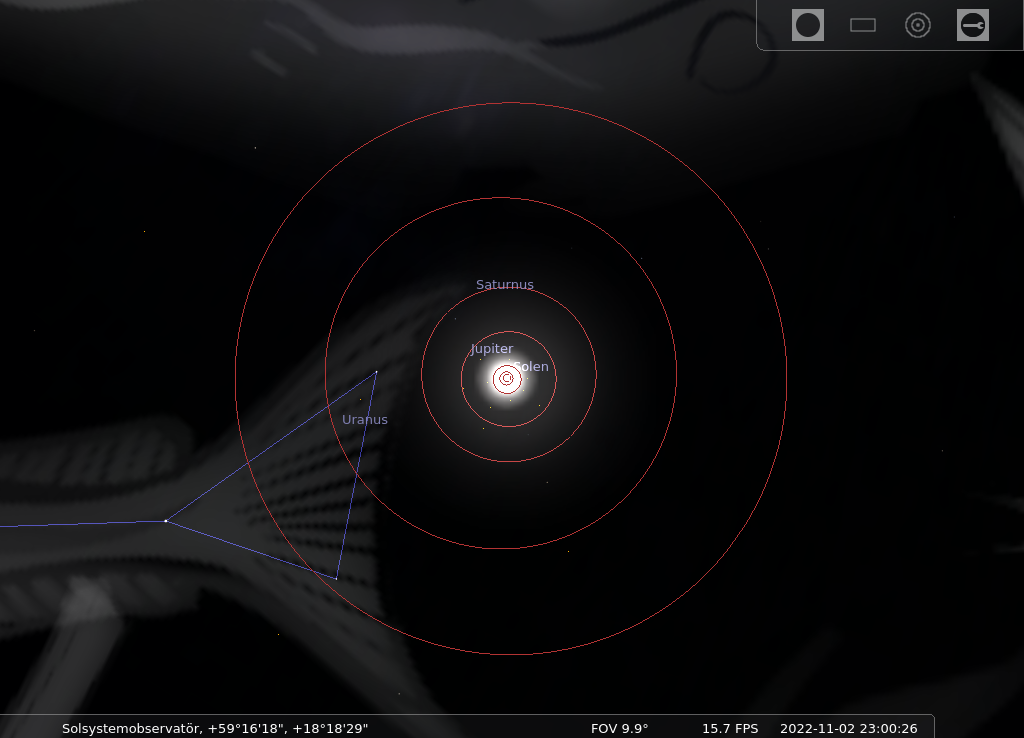
\includegraphics[scale=0.35]{stellarium-003.png}
  \caption{Planetsystemet}
  \label{fig4}
\end{figure}
Avmarkerar man att programmet endast ska visa planeter så fås elliptiska banor för något som
måste vara kometer

\begin{figure}[H]
\centering
  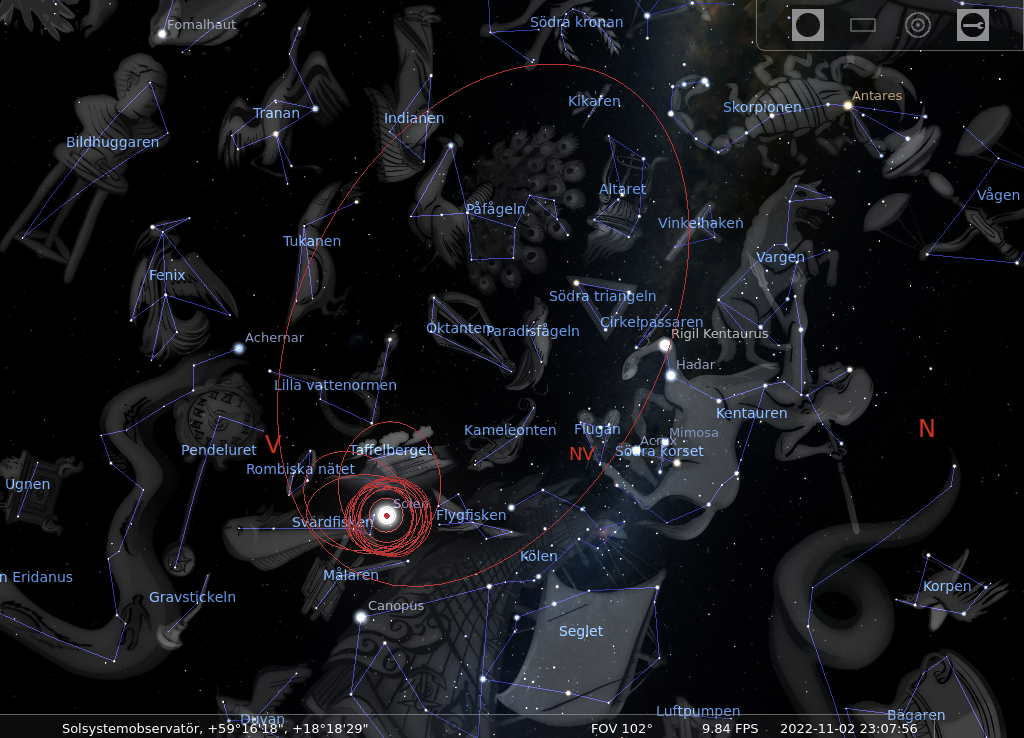
\includegraphics[scale=0.35]{stellarium-004.png}
  \caption{Solsystemet inkluderande kometer}
  \label{fig4}
\end{figure}
\item[--] Genom att öka tidens hastighet på knapplisten längst ner till höger (tryck flera gånger) så
kan du se hur planeterna rör sig. När kommer jorden och Mars att vara så nära varandra de
kan nästa gång?\\
De närmsta datumen då jorden kommer att vara nära Mars är 2022-12-15 och 2025-01-24
\begin{figure}[H]
\centering
  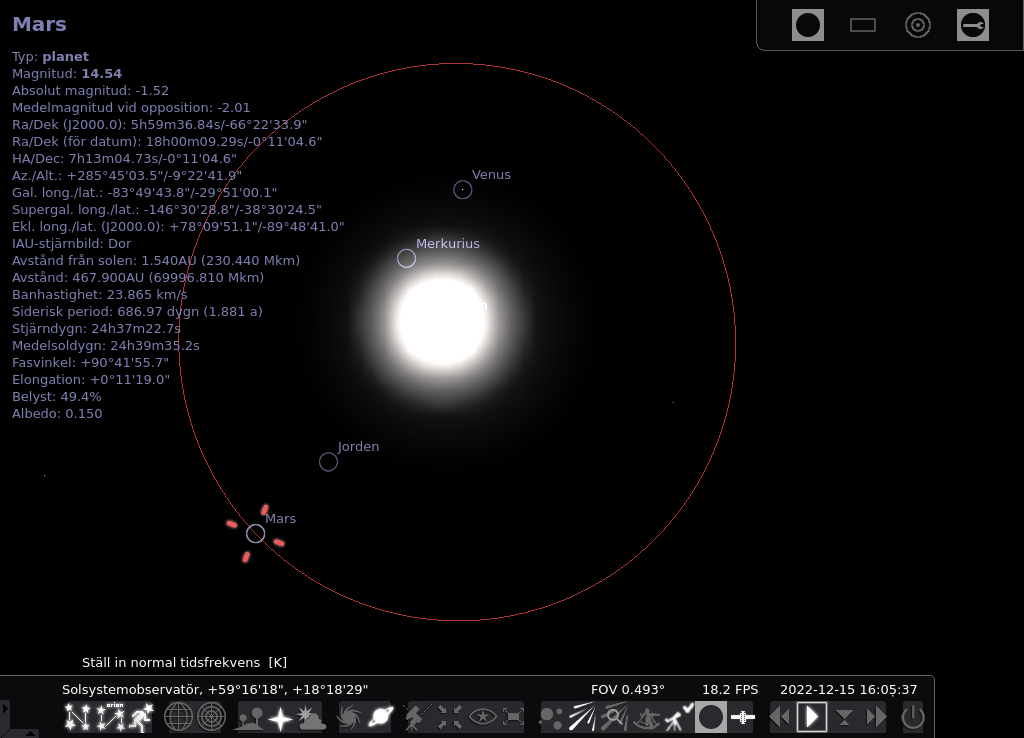
\includegraphics[scale=0.35]{stellarium-006.png}
  \caption{Mars nära jorden 2022-12-15}
  \label{fig4}
\end{figure}
\begin{figure}[H]
\centering
  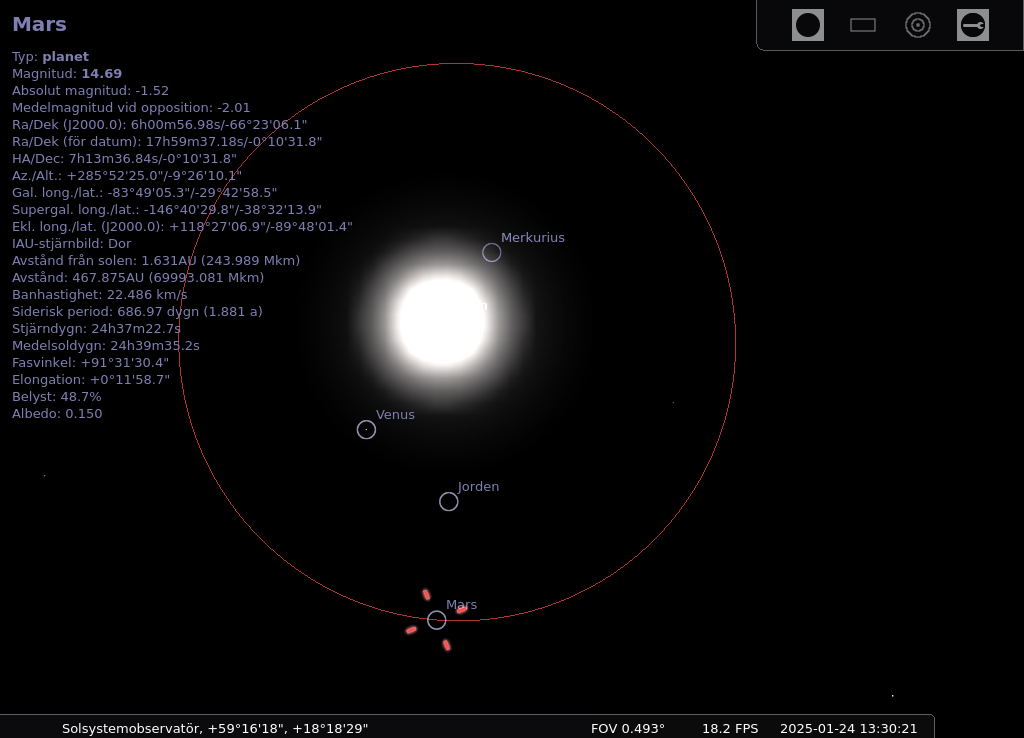
\includegraphics[scale=0.35]{stellarium-005.png}
  \caption{Mars nära jorden 2025-01-24}
  \label{fig4}
\end{figure}
Mars var dock extremt nära jorden 2020-10-16 (se bild nedan) som är runt den tidpunkten labbkompendiet skrevs
och som förmodligen är jämförelseavståndet
\begin{figure}[H]
\centering
  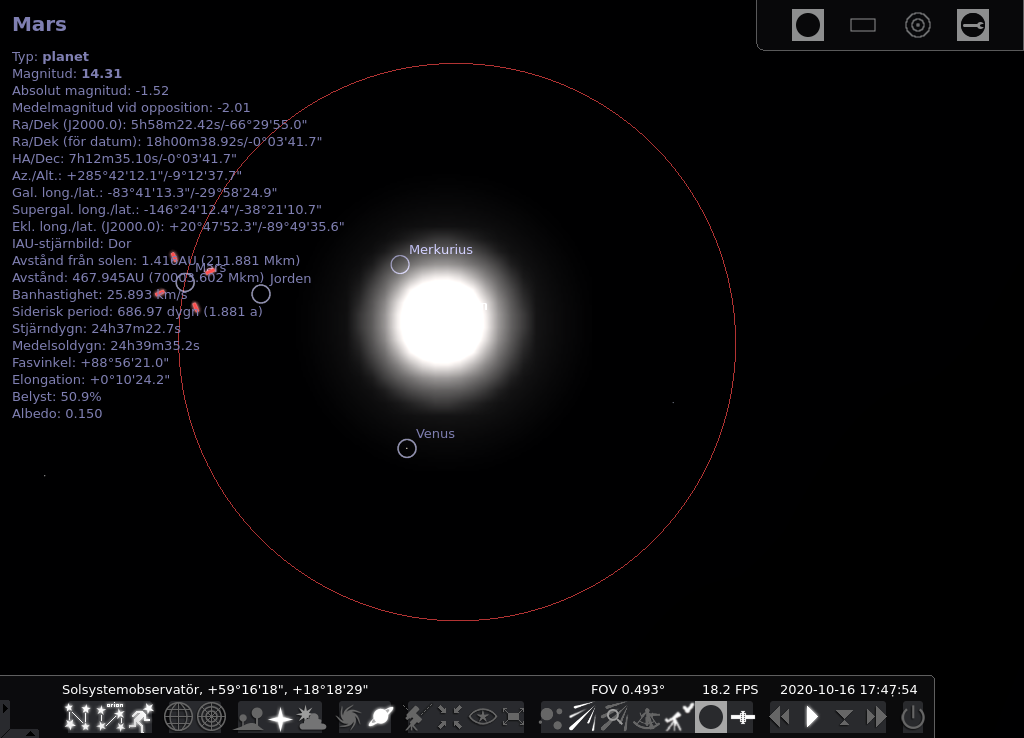
\includegraphics[scale=0.35]{stellarium-008.png}
  \caption{Mars nära jorden 2020-10-16}
  \label{fig4}
\end{figure}

\item[--] Hur rör sig Mars i förhållande till stjärnorna? \\
Den gör ``knixar'' då och då dvs. rör sig tillbaka innan den fortsätter framåt

\begin{figure}[H]
\centering
  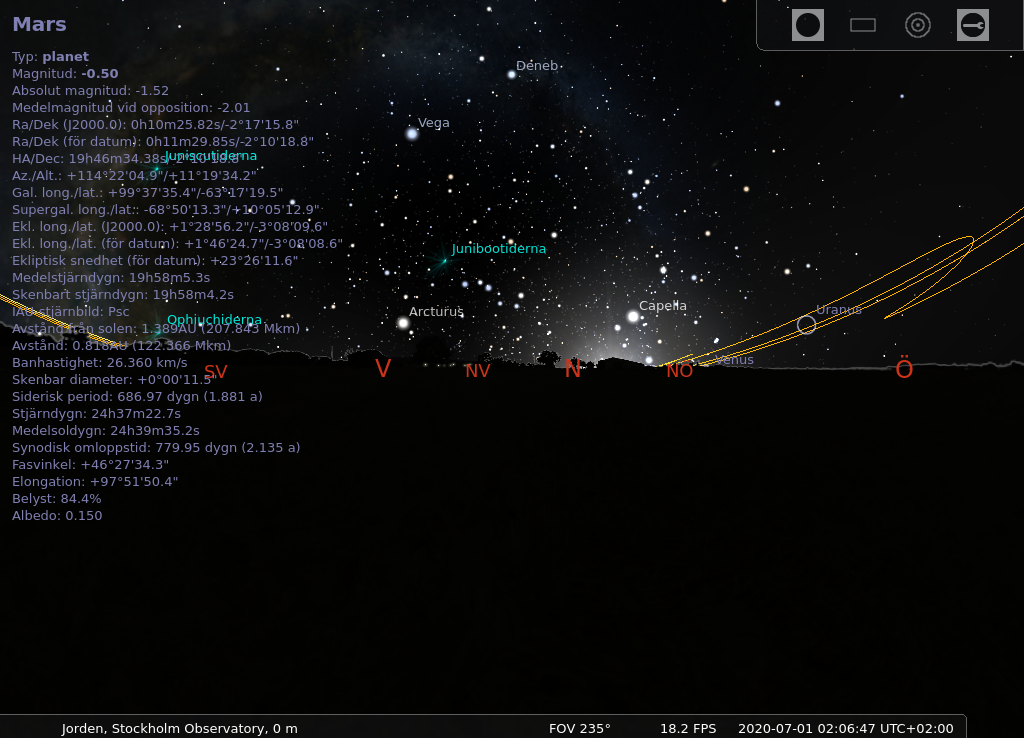
\includegraphics[scale=0.35]{stellarium-011.png}
  \caption{Trackingspår av Mars bana som påvisar retrograd rörelse}
  \label{fig4}
\end{figure}



\item[--] Hur rör sig planeterna? Vilka kan ibland ha en retrograd rörelse, dvs ibland skenbart börja
röra sig åt motsatt håll?\\
För samtliga planeter utanför jordbanan kan retrograd rörelse ses och bör också
kunna ses för månen.

\item[--] Vad beror denna effekt på? Ett historiskt problem!\\
Detta beror på exempelvis jorden kommer ifatt planeter, hinner upp dem och åker ifrån dem i sin bana relativt planeterna\footnote{By Brian Brondel - Own work, CC BY-SA 3.0, \url{https://commons.wikimedia.org/w/index.php?curid=1652425}}
men fenomenet är inte synbart särskilt väl för en planet som har en inre bana eftersom det innebär
att titta mot solen. Möjligtvis kan detta vara möjligt korta studner i under soluppgång och solnedgång.
Fenomenet tydligast för planeten Mars som är närmast därför att parallaxeffekten blir som störst
och avtar sedan med avståndet från jordbanan utåt sett.

\begin{figure}[H]
\centering
 \includesvg[scale=0.9]{Retrograde_Motion.bjb.svg}
  \caption{Trackingspår av Mars bana som påvisar retrograd rörelse}
  \label{fig4}
\end{figure}


\end{itemize}
\newpage
\section{Solförmörkelser}

\begin{itemize}
    \item[--] Mexico City 1991-07-11
\begin{figure}[H]
\centering
  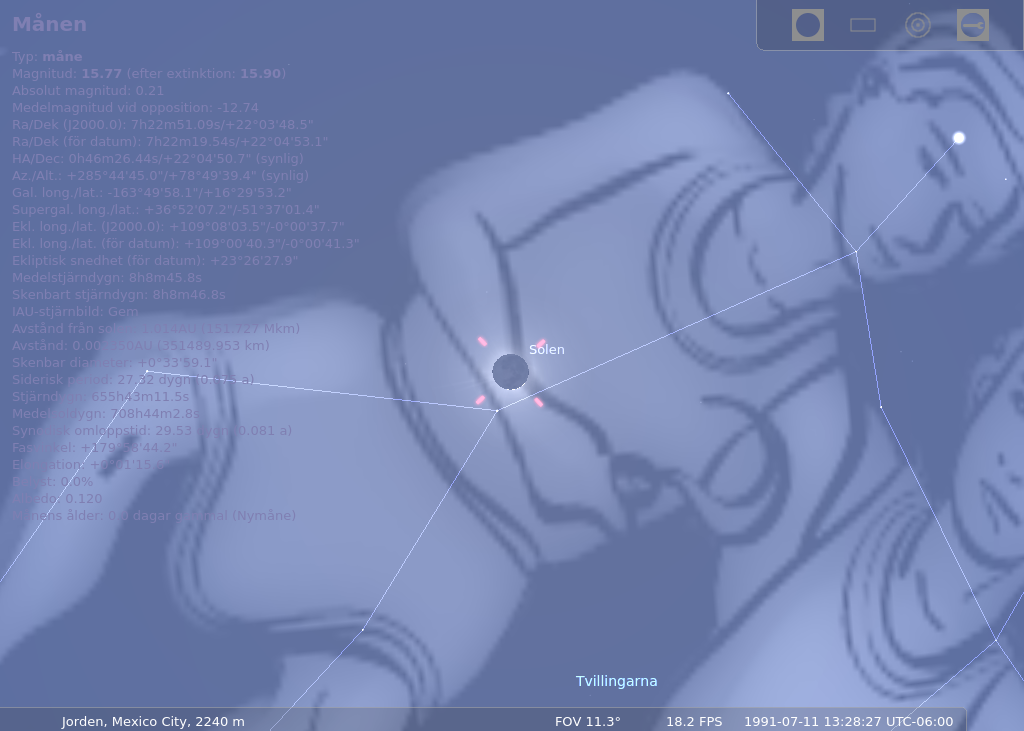
\includegraphics[scale=0.34]{stellarium-032.png}
  \caption{Mexico City 1991-07-11, kl. 13:28:27}
  \label{fig4}
\end{figure}


\item[--] Paris 1999-08-11
\begin{figure}[H]
\centering
  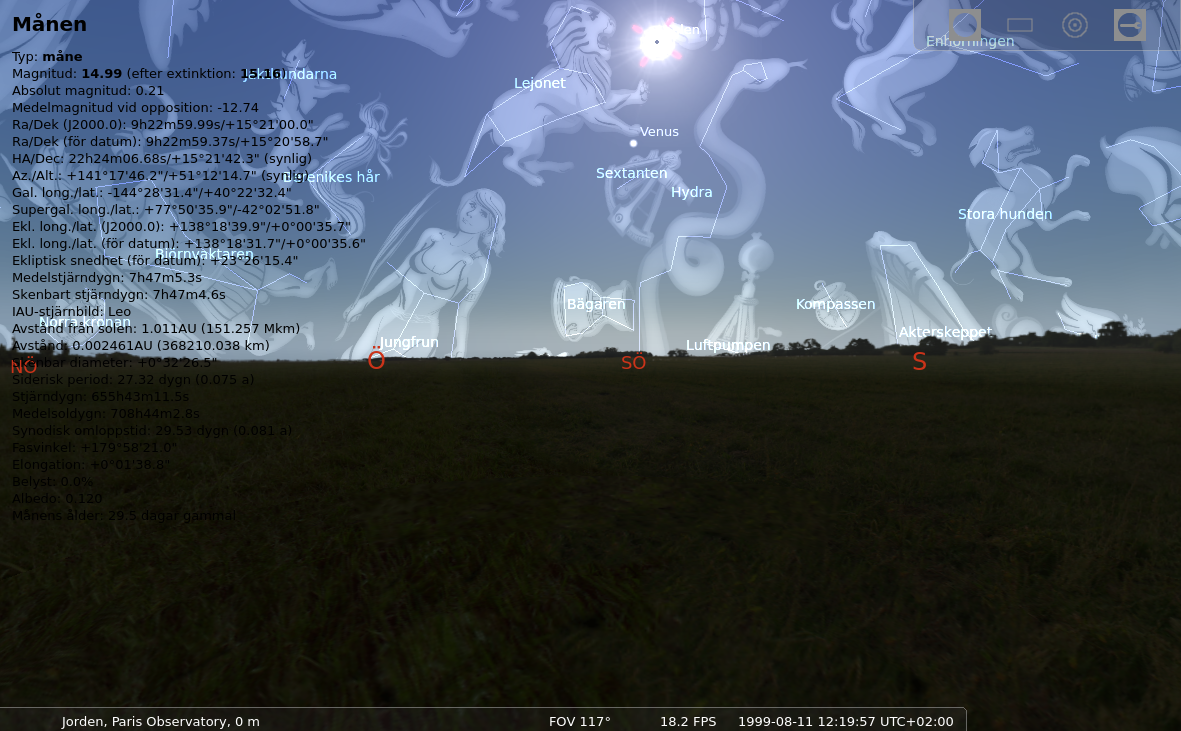
\includegraphics[scale=0.3]{stellarium-033.png}
  \caption{Paris 1999-08-11 kl. 12:19:57 }
  \label{fig4}
\end{figure}

\end{itemize}
\newpage
\section{Jupiter och dess månar}
\begin{itemize}
\item[--] Ser du skuggan av månarna?
Skuggan aven av de gallileiska månarna syns men överensstämmelse med vy såsom solsystemsobservatör
stämmer inte med jordobservatör.
Såsom solsystemsobservatör ligger Io is skugga 2022-11-05, kl. 16:19 
 \begin{figure}[H]
\centering
  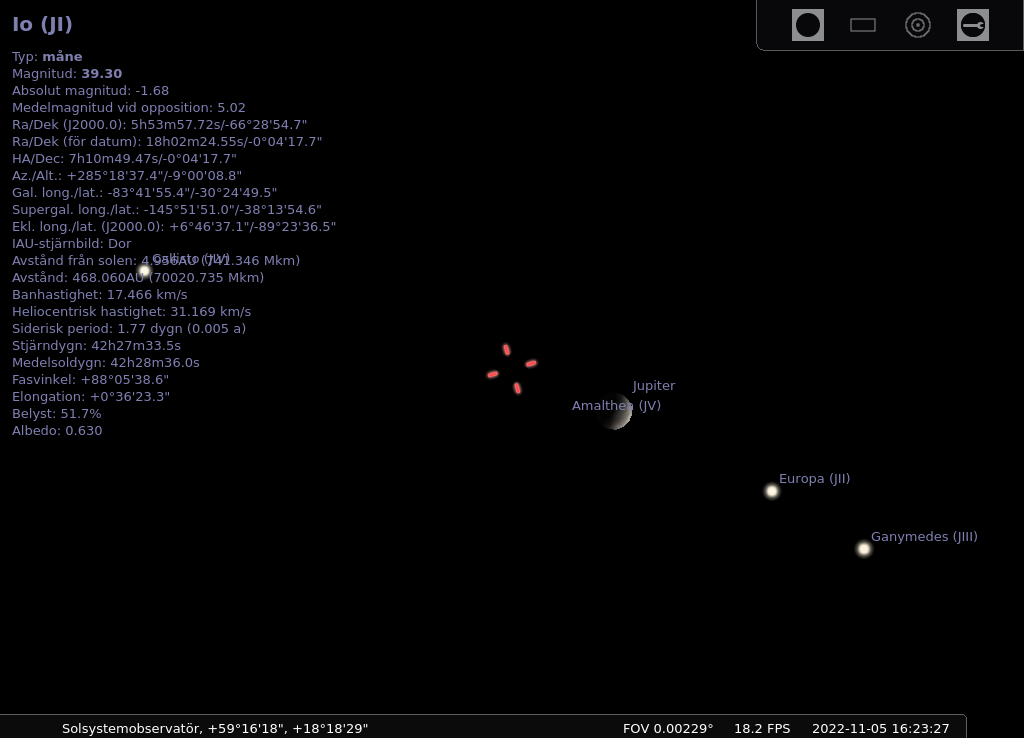
\includegraphics[scale=0.3]{stellarium-041.png}
  \caption{SSO 2022-11-05, kl. 16:19 }
  \label{fig4}
\end{figure}
medan det som jordobservatör från Stockholm ser ut att vara Ios skugga
\begin{figure}[H]
\centering
  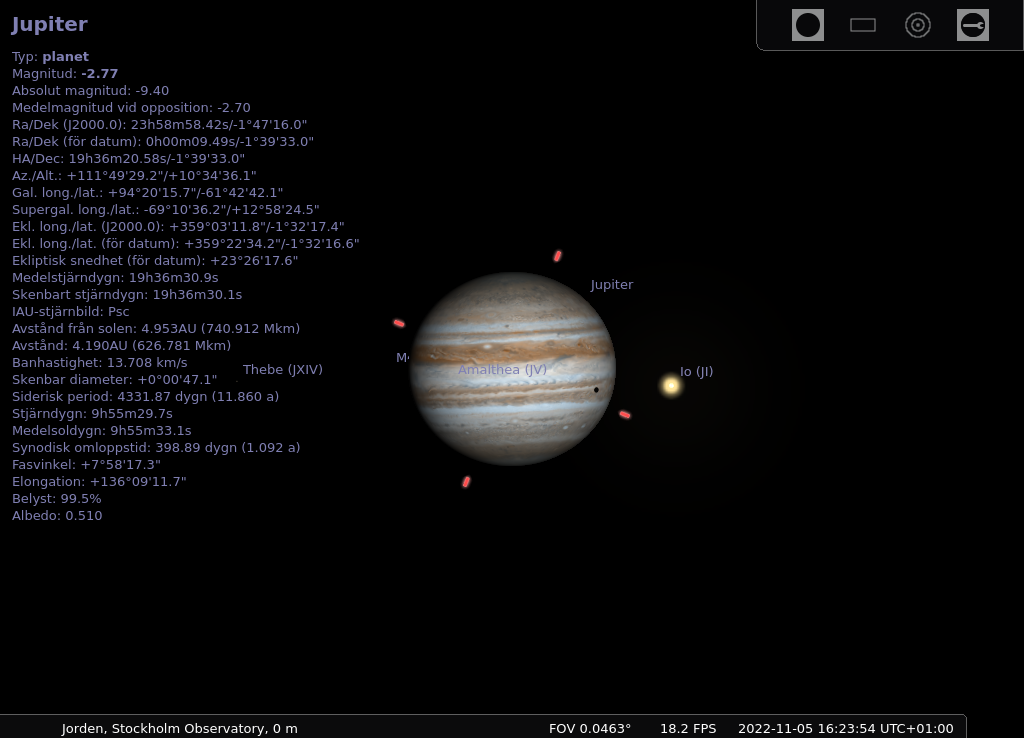
\includegraphics[scale=0.3]{stellarium-042.png}
  \caption{Jorddobservatör Stockholm, 2022-11-05, kl. 16:19 }
  \label{fig4}
\end{figure}
\item[--] Kan du få en uppfattning om Jupiters rotationstid?
Mäter tiden för den stora fläckens uppdykande i synfältet
\begin{figure}[H]
     \centering
     \begin{subfigure}[b]{0.45\textwidth}
         \centering
         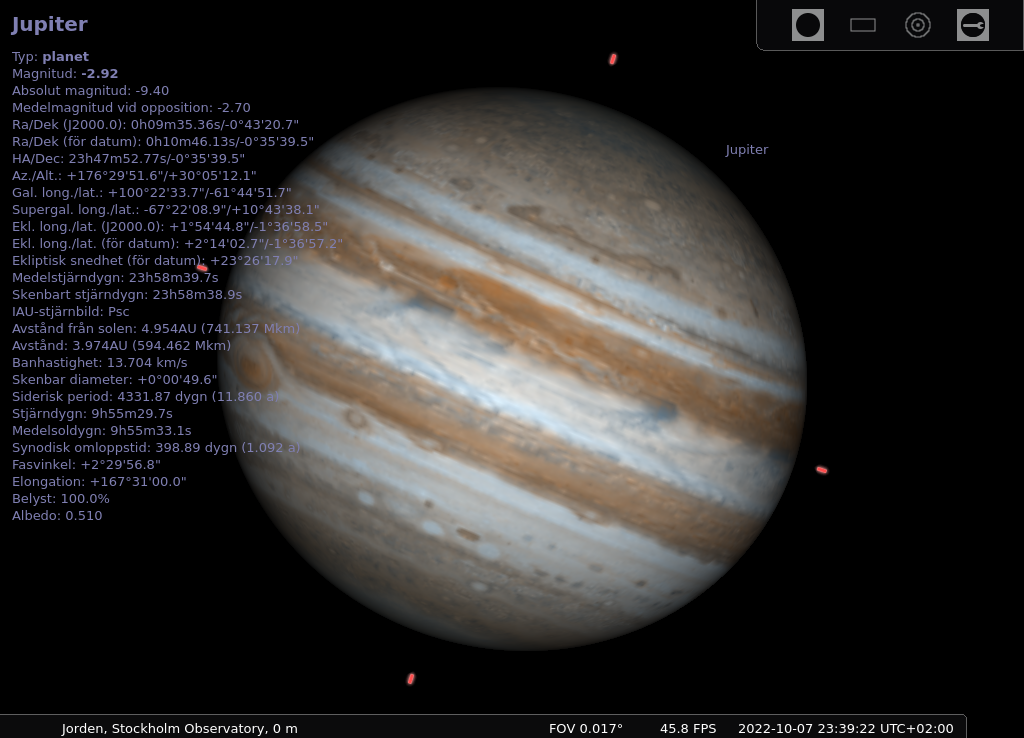
\includegraphics[width=\textwidth]{stellarium-044.png}
         \caption{2022-10-07, kl. 23:39:22}
         \label{fig:y equals x}
     \end{subfigure}
     \hfill
     \begin{subfigure}[b]{0.45\textwidth}
         \centering
         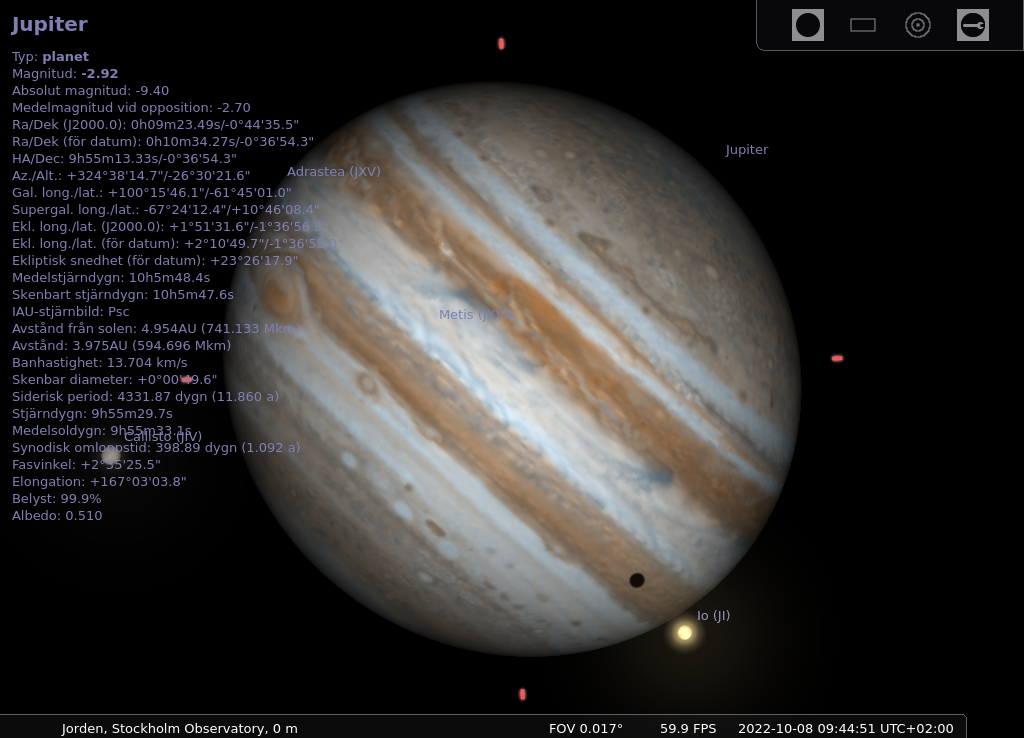
\includegraphics[width=\textwidth]{stellarium-045.png}
         \caption{2022-10-08, kl. 09:44:51}
         \label{fig:three sin x}
     \end{subfigure}
     \hfill
        \caption{Periodtid egenrotation ca 10.5 timmar}
        \label{fig:perod graphs}
\end{figure}
\item[--] Hur ligger månarna ikväll i förhållande till Jupiter och varandra?
De ser ut att vara upplinjerade på rad men Jupiters skugga verkar inte överensstämma
såsom jordobservatör med SSO
\begin{figure}[htbp]
     \centering
     \begin{subfigure}[b]{0.45\textwidth}
         \centering
         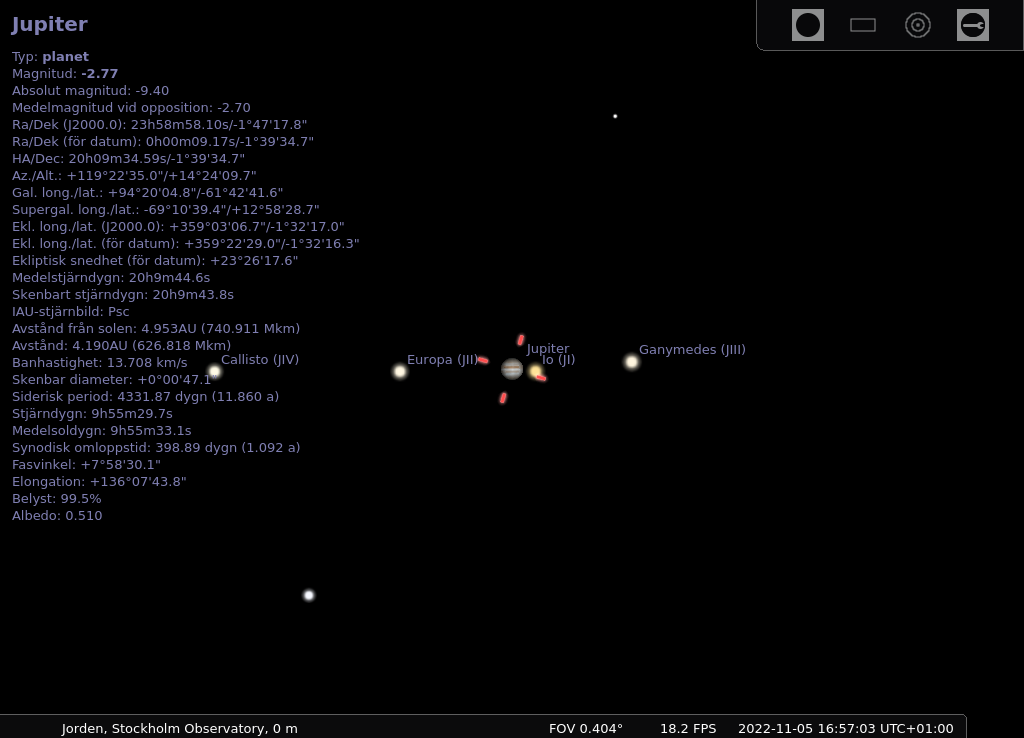
\includegraphics[width=\textwidth]{stellarium-046.png}
         \caption{Stockholm, 2022-11:05, kl. 16:57:03}
         \label{fig:y equals x}
     \end{subfigure}
     \hfill
     \begin{subfigure}[b]{0.45\textwidth}
         \centering
         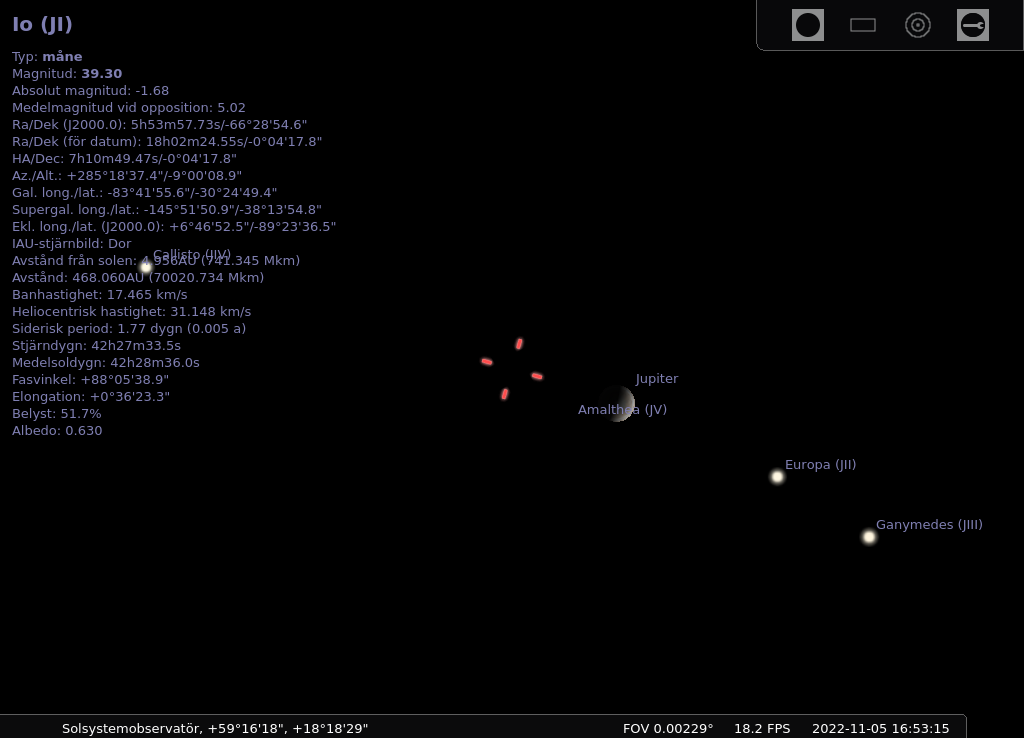
\includegraphics[width=\textwidth]{stellarium-048.png}
         \caption{SSO, 2022-11:05, kl. 16:53:15}
         \label{fig:three sin x}
     \end{subfigure}
     \hfill
        \caption{Jupiter med de gallileiska månarna Io, Callisto, Ganymedes och Europa}
        \label{fig:perod graphs}
\end{figure}
\newpage
\item[--] Kan man se planeten ikväll/i natt i verkligheten?
Tror att det är Jupiter men det stämmer inte riktigt med Stellarium.
Kommentera gärna därför att jag har aldrig sett en planet i verkligheten.
Fjärdhundra har GPS koordinater $59^\circ 46' 35.4''\text{N}$ $16^\circ 55' 13.476''\text{E}$
\begin{figure}[H]
\centering
  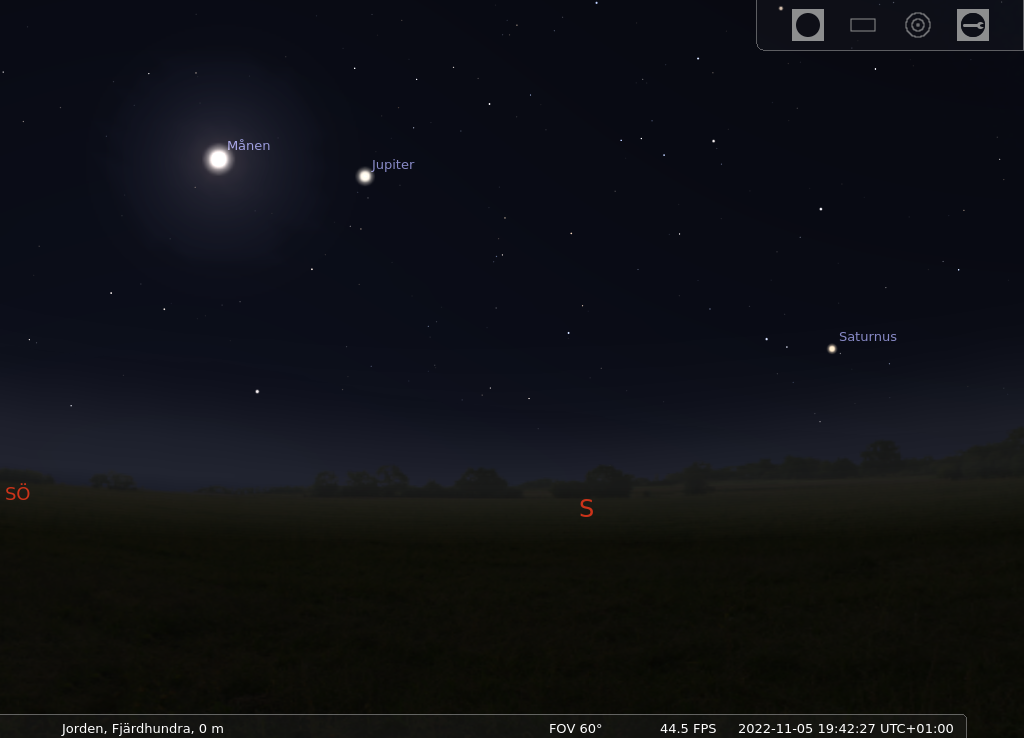
\includegraphics[scale=0.3]{stellarium-049.png}
  \caption{Fjärdhundra 2022-11-05, kl. 19:27 }
  \label{fig4}
\end{figure}

\begin{figure}[H]
\centering
  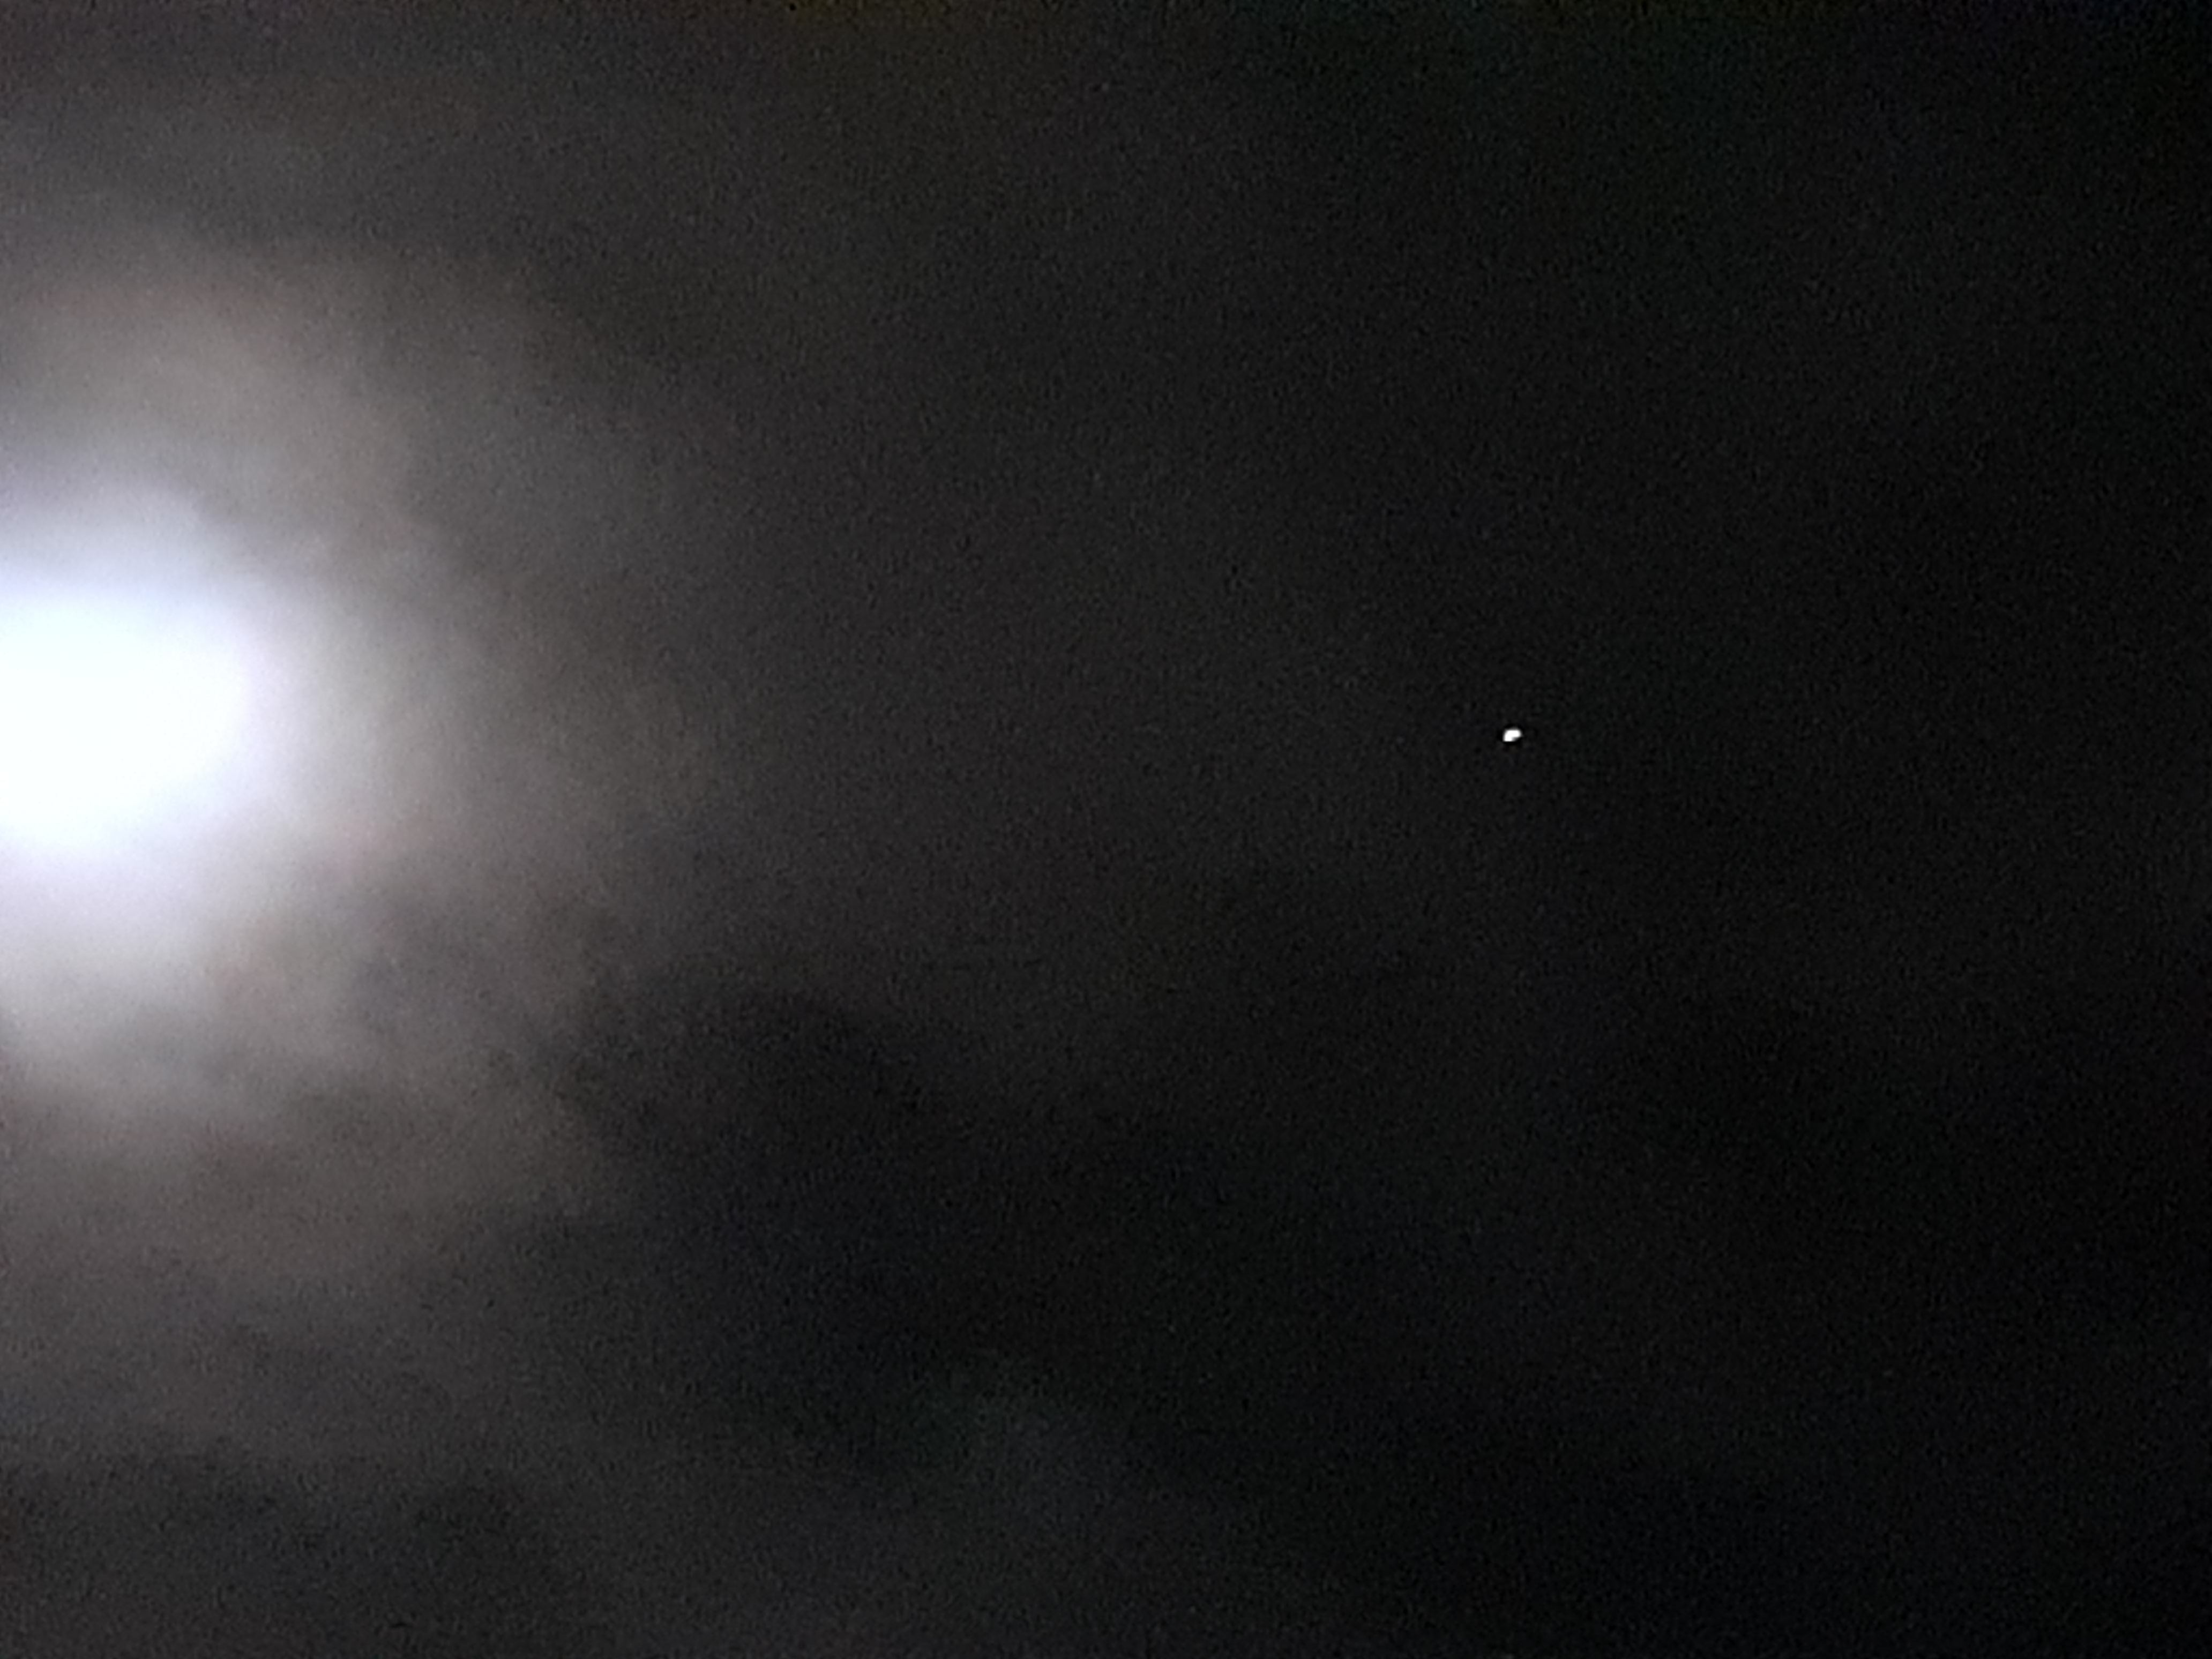
\includegraphics[scale=0.1]{20221105_194014.jpg}
  \caption{Fjärdhundra 2022-11-05, kl. 19:27 }
  \label{fig4}
\end{figure}
\newpage
\item[--] När kan man se planeten bäst, dvs när står den i opposition?
Jupiter kommer att stå i opposition 2023-11-10 ca kl. 20
\begin{figure}[H]
\centering
  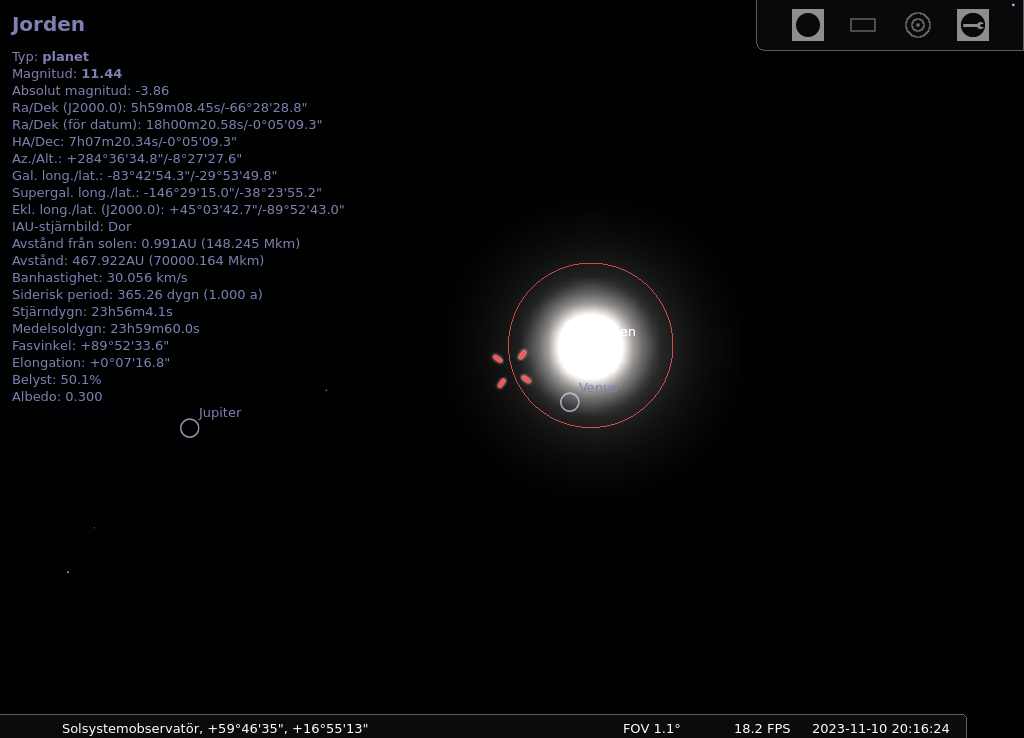
\includegraphics[scale=0.4]{stellarium-050.png}
  \caption{Jupiter i opposition 2023-11-10 ca kl. 20 }
  \label{fig4}
\end{figure}
\item[--] Hur länge dröjer det mellan de tillfällen då Jupiter står i opposition?
Sist Jupiter stod i opposition var en månad sedan, vilket betyder ca 13 månader emellan.
\begin{figure}[H]
\centering
  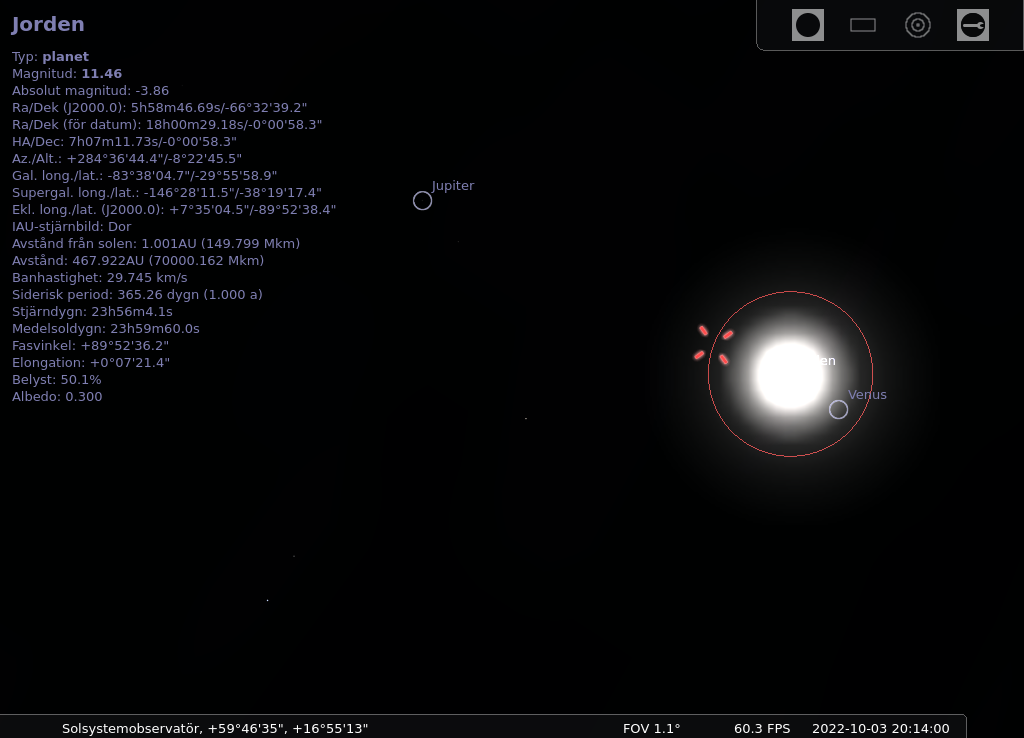
\includegraphics[scale=0.4]{stellarium-053.png}
  \caption{Jupiter i opposition 2022-10-03 ca kl. 20 }
  \label{fig4}
\end{figure}
\end{itemize}

\newpage
\section{Månen}

\begin{itemize}
\item[--] Hur ser den ut denna kväll?(Stockholm den 13 feb 2020 kl 17.50) Är det fullmåne?
Nej det är mer som en halvmåne och den ligger under horisonten ej synlig
\begin{figure}[H]
\centering
  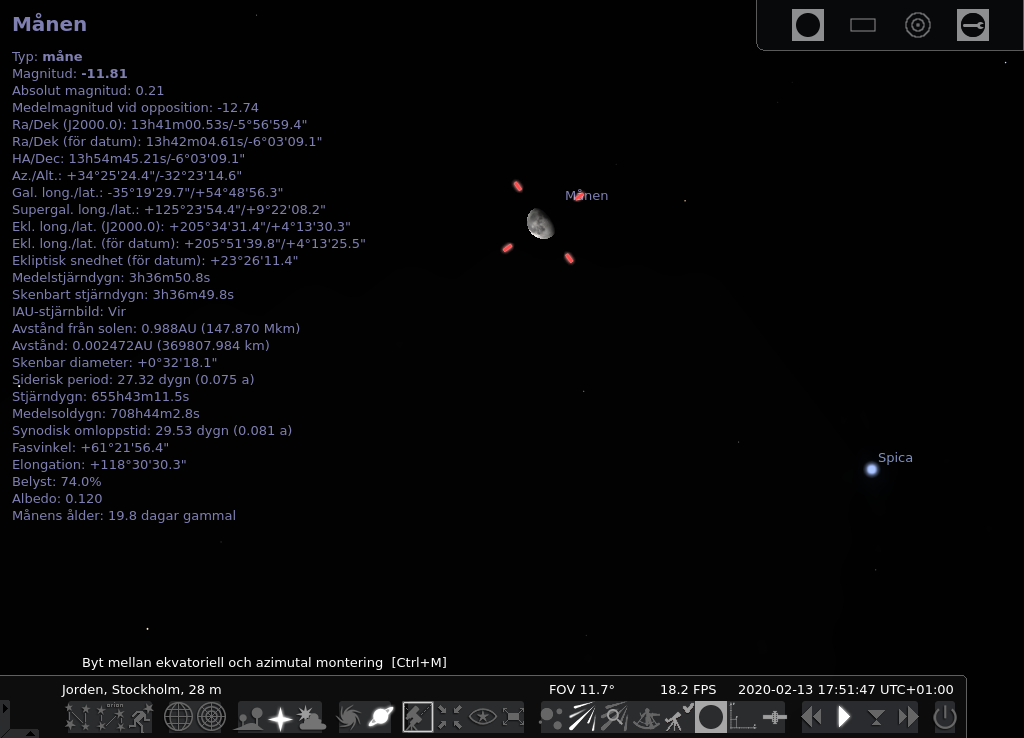
\includegraphics[scale=0.4]{stellarium-054.png}
  \caption{Halmvmåne under horisonten, Stockholm, 2020-02-13, kl. 17:50 }
  \label{fig4}
\end{figure}
Startar multipla instanser av Stellarium med kommandot 
\verb+nohup dbus-run-session stellarium &+\\
Plugin ``Remote Sync'' tillåter
automatisk kopiering inställningar från en instans av Stellarium til en annan. I detta
fall har endast tidssynkronisering aktiverats som dock inte fungerar korrekt
för instansen som är SSO.

\begin{figure}[htbp]
     \centering
     \begin{subfigure}[b]{0.45\textwidth}
         \centering
         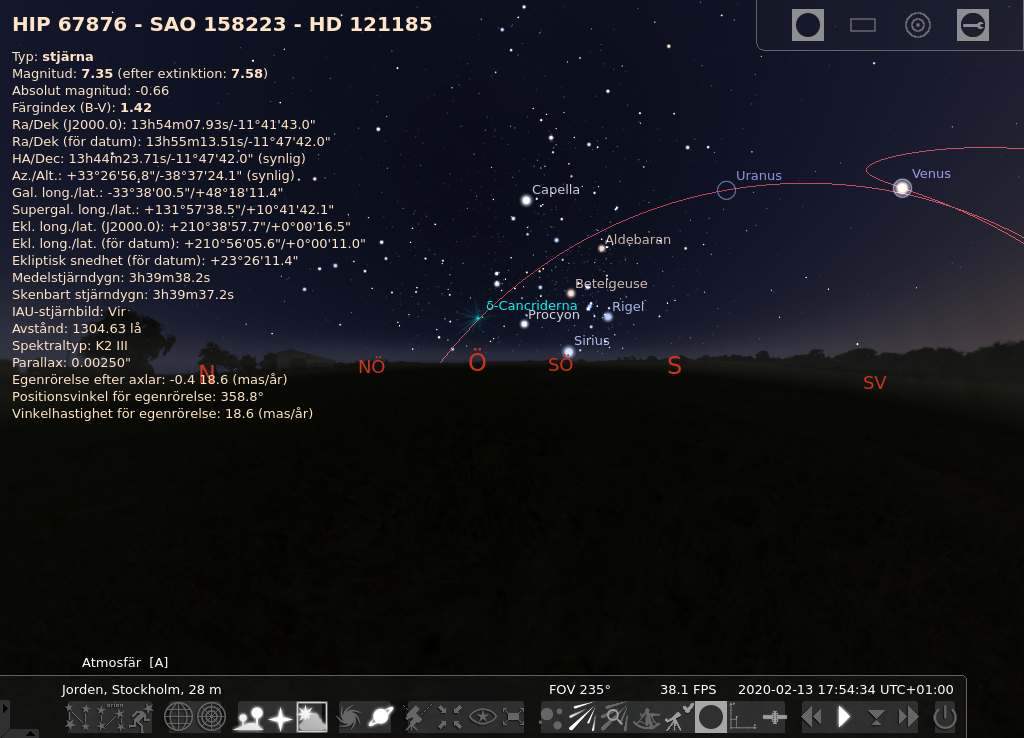
\includegraphics[width=\textwidth]{stellarium-055.png}
         \caption{Månen under horisonten, Stockholm, 2020-02-13, kl. 17:50}
         \label{fig:y equals x}
     \end{subfigure}
     \hfill
     \begin{subfigure}[b]{0.45\textwidth}
         \centering
         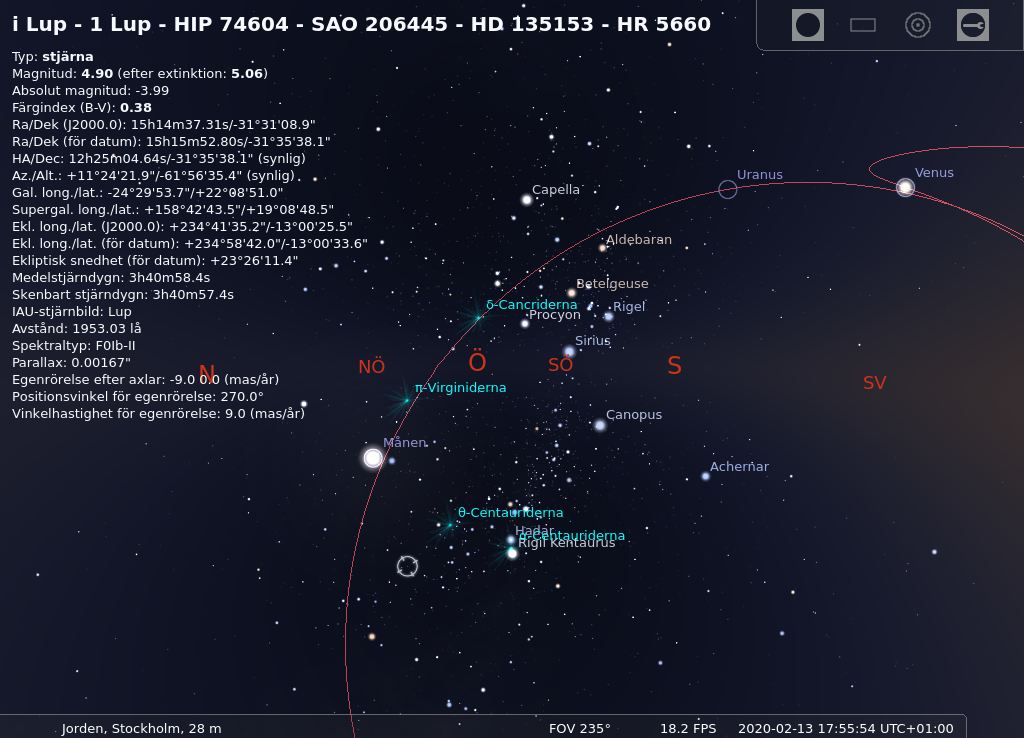
\includegraphics[width=\textwidth]{stellarium-056.png}
         \caption{Transparant jord - måne synlig, Stockholm, 2020-02-13, kl. 17:50}
         \label{fig:three sin x}
     \end{subfigure}
     \hfill
        \caption{Kollage Stockholm, 2020-02-13, kl. 17:50 }
        \label{fig:perod graphs}
\end{figure}
\item[--] Undersök nu hur månen ändrar sitt läge och fas under en månads tid. Flytta fram en dag åt
gången (med Datum/tid).  

\begin{figure}[H]
     \centering
     \begin{subfigure}[b]{0.45\textwidth}
         \centering
         \includegraphics[width=\textwidth]{Stellarium/Unix_stellarium-000.png}
         \caption{SSO utzoomad 2020-02-13, kl. 17:50}
         \label{fig:y equals x}
     \end{subfigure}
     \hfill
     \begin{subfigure}[b]{0.45\textwidth}
         \centering
         \includegraphics[width=\textwidth]{Stellarium/Unix_stellarium-001.png}
         \caption{SSO 2020-02-13, kl. 17:50}
         \label{fig:three sin x}
     \end{subfigure}
     \hfill
        \caption{Kollage Solsystemobservatör, 2020-02-13, kl. 17:50 }
        \label{fig:perod graphs}
\end{figure}



\item[--] Hur rör sig månen över himlen under månaden?\\
Månen rör sig upp och ner över ekvatorn vilket gör att den stiger upp och ner över horisonten i en båg
formad bana.
\item[--] Hur ändrar sig månfasen? \\
Stellarium har gjort felet att de använder sig av foton på månen istället för raytracing av
 virutella modeller vilket gör att nymåne infaller för tidigt jämför med om man är SSO.
Fullmåne inträffar ungerfär där man förväntar sig att Waning Gibbons är.\\
\newpage
\textit{\textbf{Waxing Gibbons}}
\begin{figure}[H]
     \centering
     \begin{subfigure}[b]{0.45\textwidth}
         \centering
         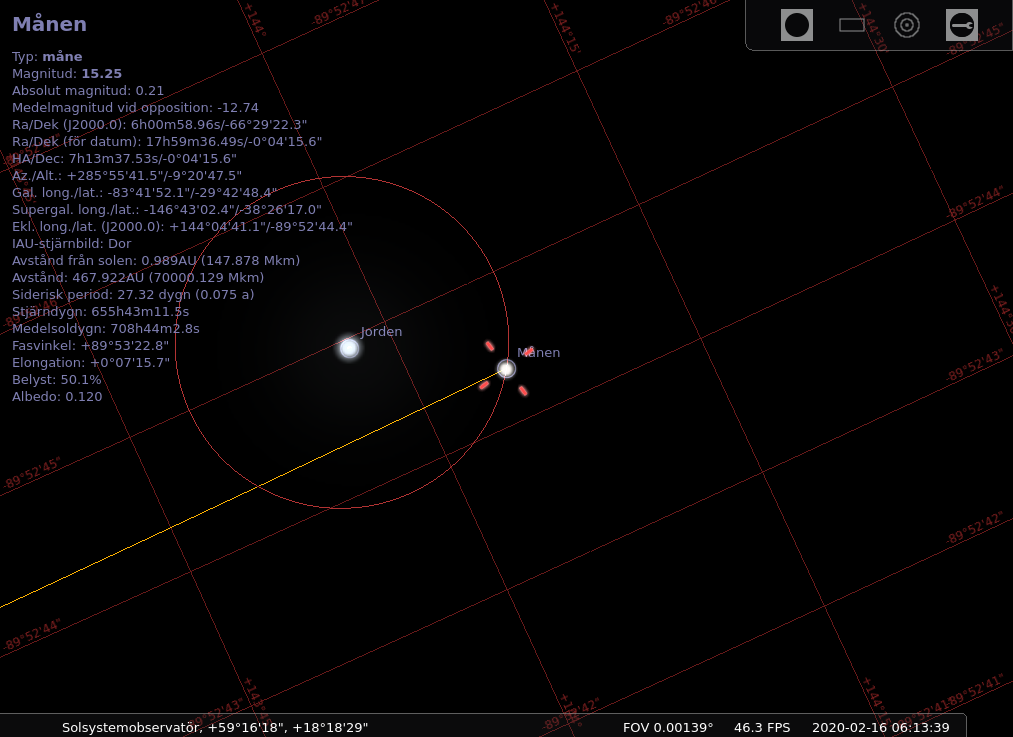
\includegraphics[width=\textwidth]{Stellarium1/WXGib/stellarium-000.png}
         \caption{SSO, 2020-02-16, kl.06:13}
         \label{fig:y equals x}
     \end{subfigure}
     \hfill
     \begin{subfigure}[b]{0.45\textwidth}
         \centering
         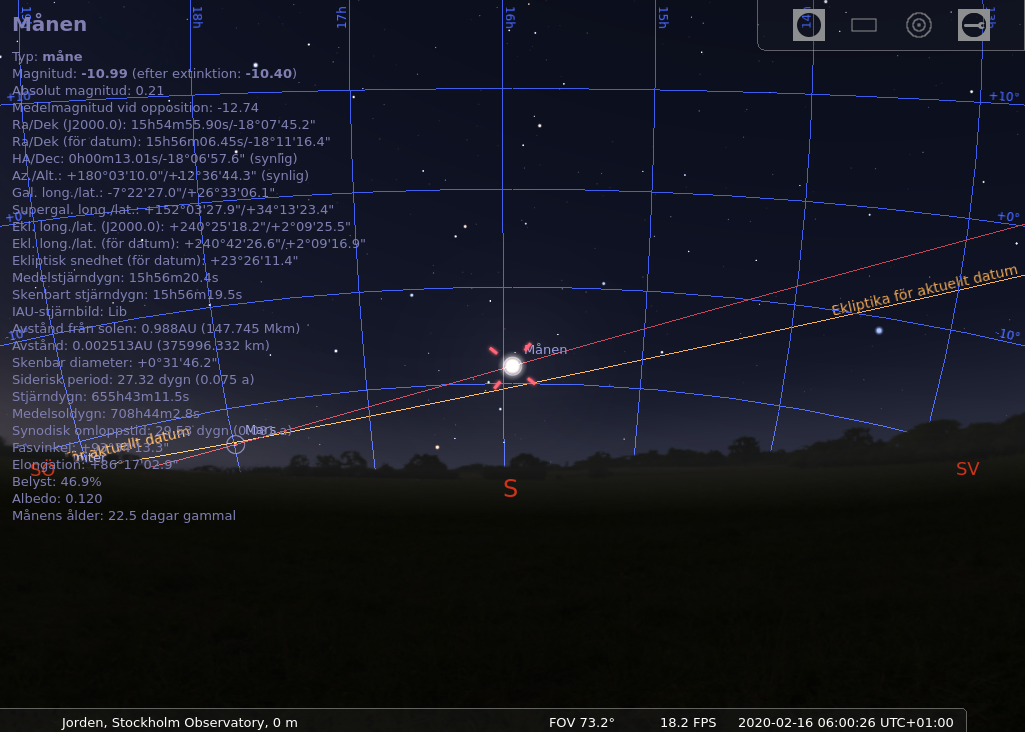
\includegraphics[width=\textwidth]{Stellarium1/WXGib/stellarium-001.png}
         \caption{Stockholm, 2020-02-16, kl.06:00 }
         \label{fig:three sin x}
     \end{subfigure}
     \hfill
     \begin{subfigure}[b]{0.45\textwidth}
         \centering
         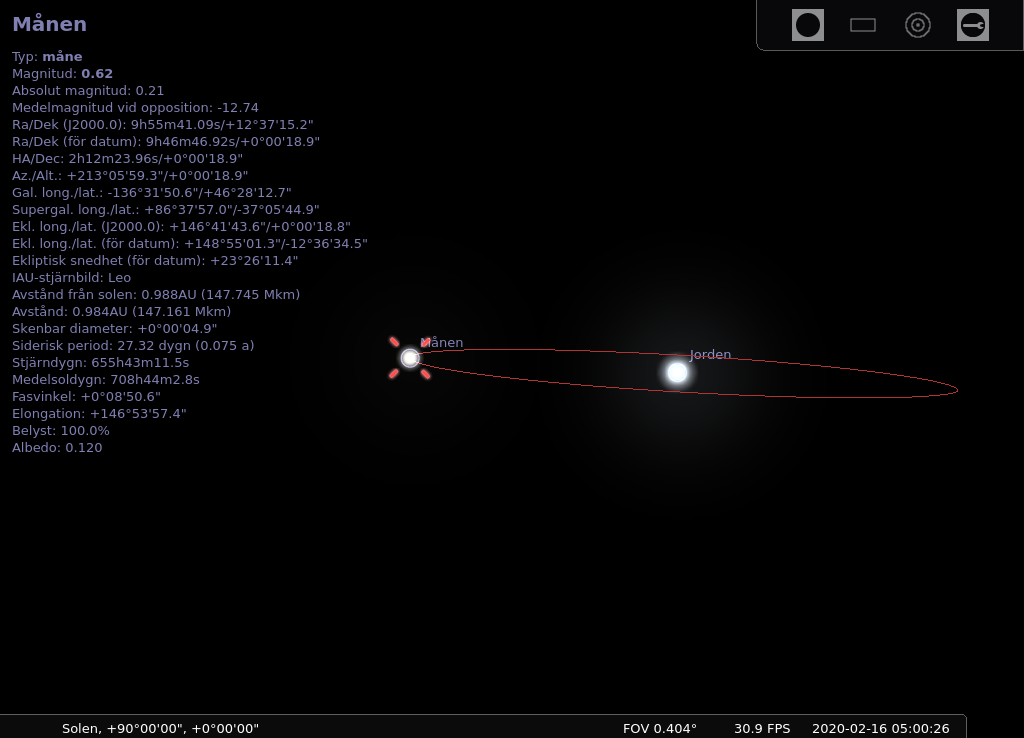
\includegraphics[width=\textwidth]{Stellarium1/WXGib/stellarium-002.png}
         \caption{Observatör solens nordpol,2020-02-16, kl. 05:00}
         \label{fig:three sin x}
     \end{subfigure}
     \hfill
     \begin{subfigure}[b]{0.45\textwidth}
         \centering
         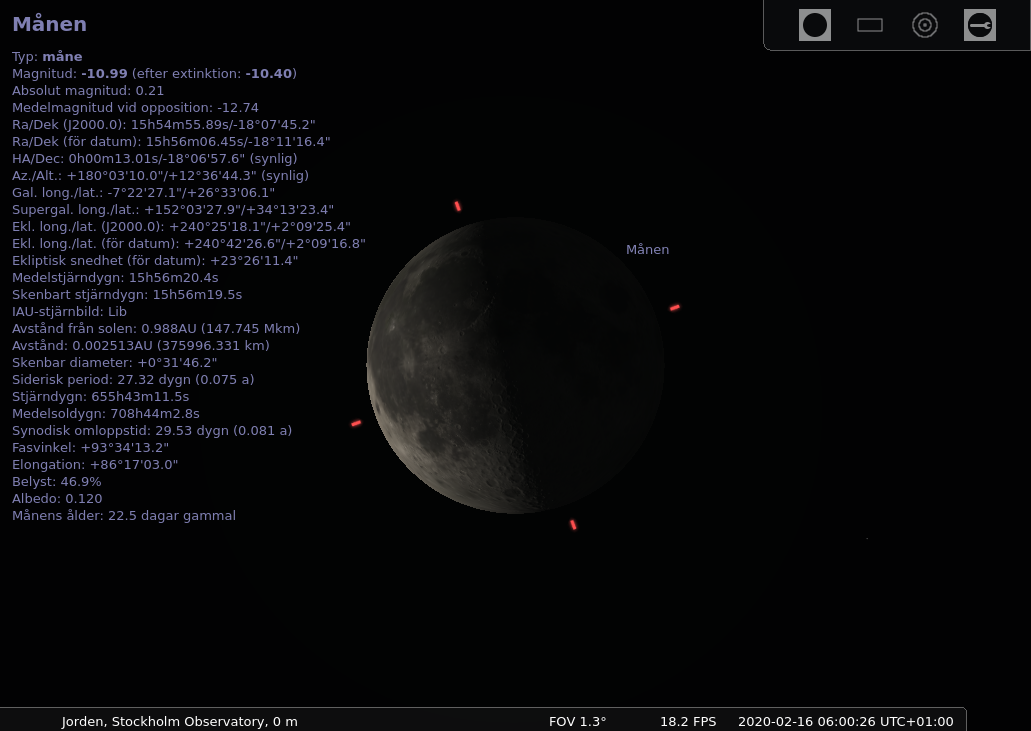
\includegraphics[width=\textwidth]{Stellarium1/WXGib/stellarium-003.png}
         \caption{Stockholm, 2020-02-16, kl. 06:00}
         \label{fig:three sin x}
     \end{subfigure}
     \hfill
        \caption{ Waxing Gibbons måne, notera tidssynk problem i Steellarium}
        \label{fig:perod graphs}
\end{figure}
\newpage
\textit{\textbf{Tredje kvarten}}
\begin{figure}[H]
     \centering
     \begin{subfigure}[b]{0.45\textwidth}
         \centering
         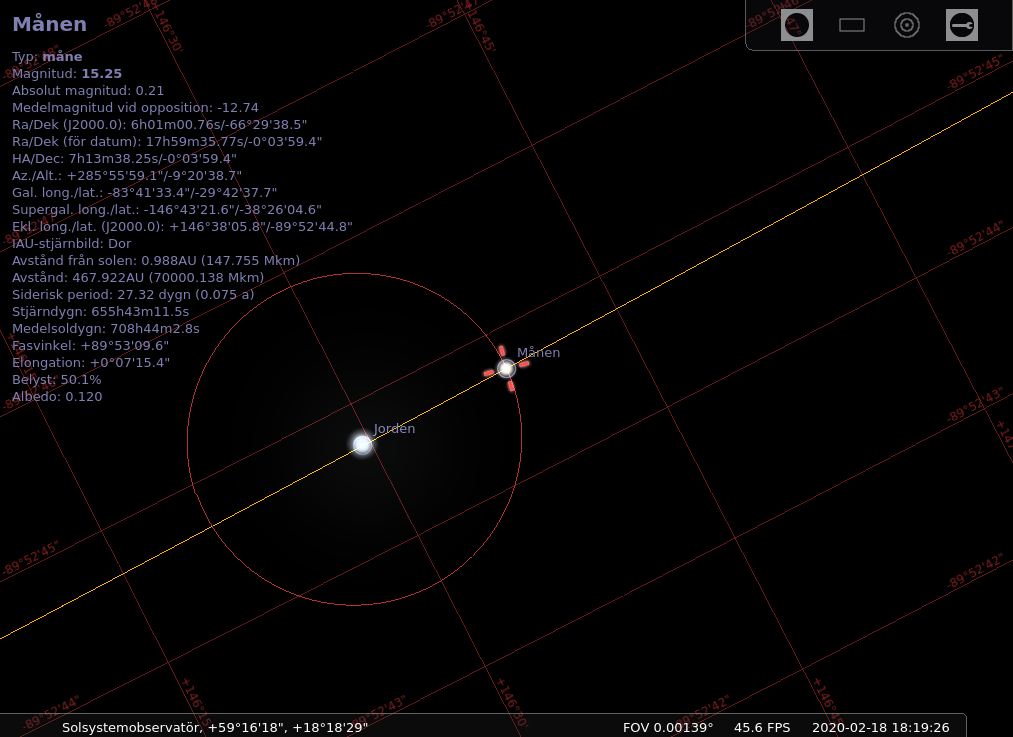
\includegraphics[width=\textwidth]{Stellarium1/3rdQ/stellarium-000.png}
         \caption{SSO, 2020-02-18, kl. 18:19}
         \label{fig:y equals x}
     \end{subfigure}
     \hfill
     \begin{subfigure}[b]{0.45\textwidth}
         \centering
         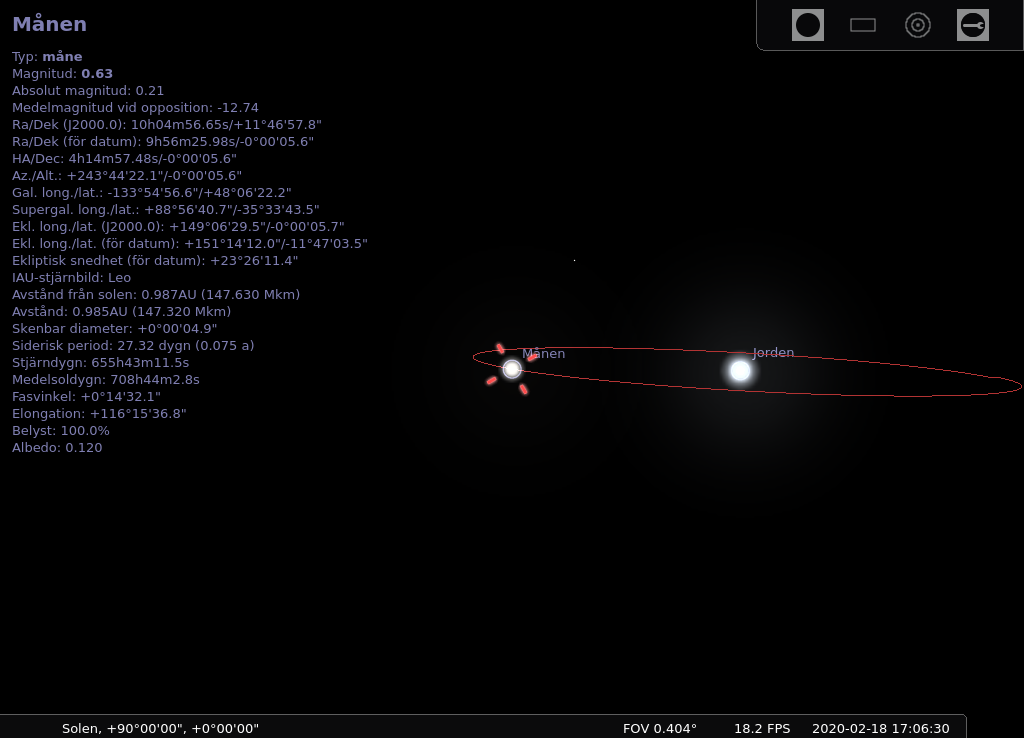
\includegraphics[width=\textwidth]{Stellarium1/3rdQ/stellarium-001.png}
         \caption{Observatör solens nordpol, 2020-02-18, kl. 17:06}
         \label{fig:three sin x}
     \end{subfigure}
     \hfill
     \begin{subfigure}[b]{0.45\textwidth}
         \centering
         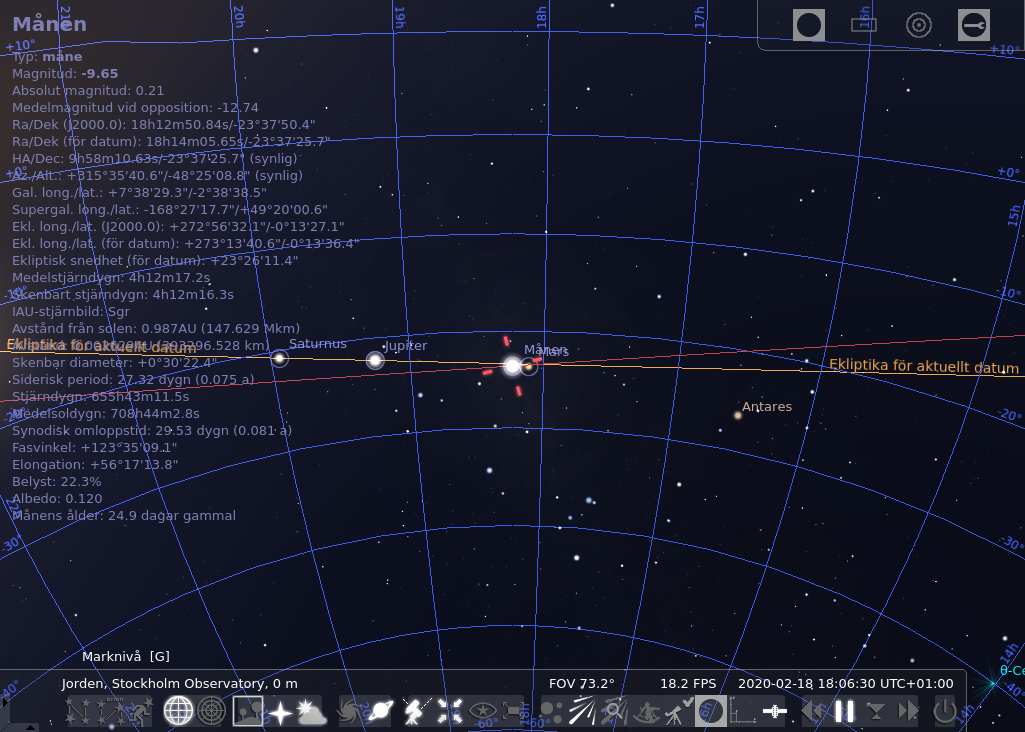
\includegraphics[width=\textwidth]{Stellarium1/3rdQ/stellarium-002.png}
         \caption{Månen under horisonten korsar ekliptikan }
         \label{fig:three sin x}
     \end{subfigure}
     \hfill
     \begin{subfigure}[b]{0.45\textwidth}
         \centering
         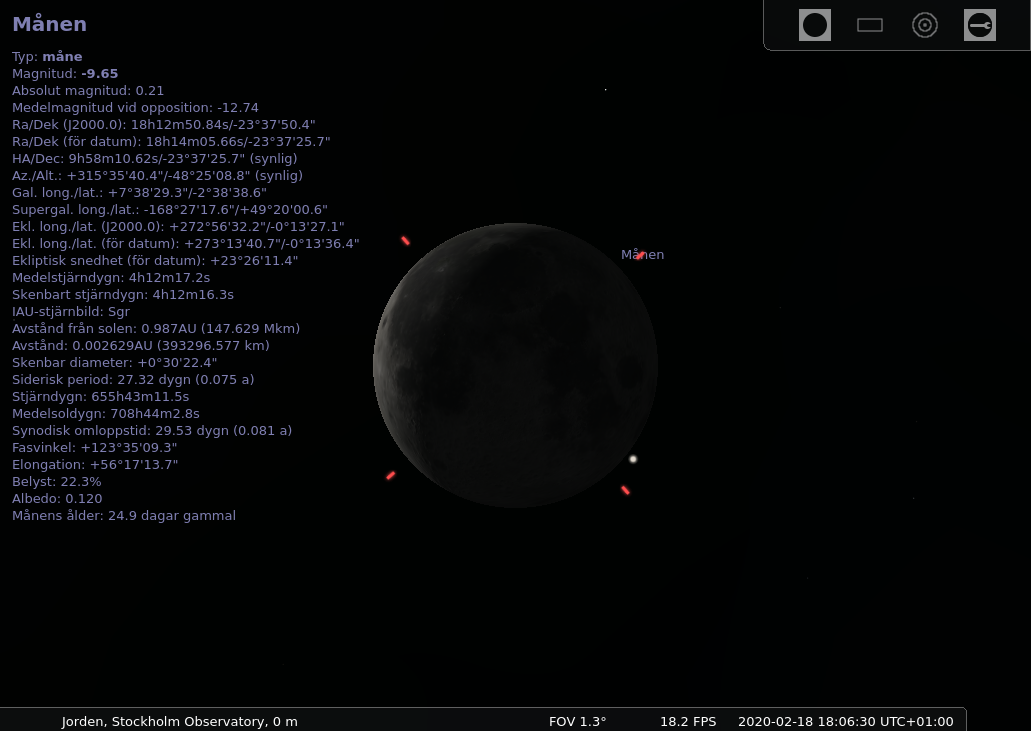
\includegraphics[width=\textwidth]{Stellarium1/3rdQ/stellarium-003.png}
         \caption{Månen sedd från Stokholm. Transparent jord}
         \label{fig:three sin x}
     \end{subfigure}
     \hfill
     \begin{subfigure}[b]{0.45\textwidth}
         \centering
         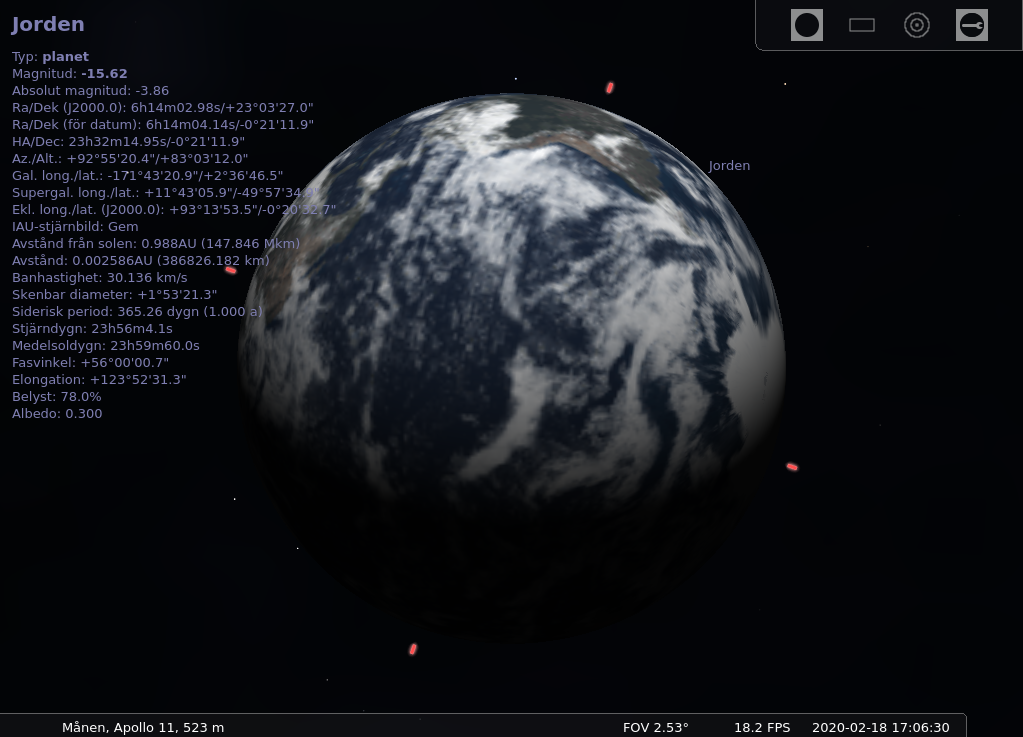
\includegraphics[width=\textwidth]{Stellarium1/3rdQ/stellarium-005.png}
         \caption{Jorden sedd från månens nordpol}
         \label{fig:three sin x}
     \end{subfigure}
     \hfill
        \caption{ Tredje kvarten}
        \label{fig:perod graphs}
\end{figure}
Notera tidsynkningsproblem hos Stellarium pluginet ``Remote Sync''
\newpage
\textit{\textbf{Waxing Crescent måne}}
\begin{figure}[H]
     \centering
     \begin{subfigure}[b]{0.45\textwidth}
         \centering
         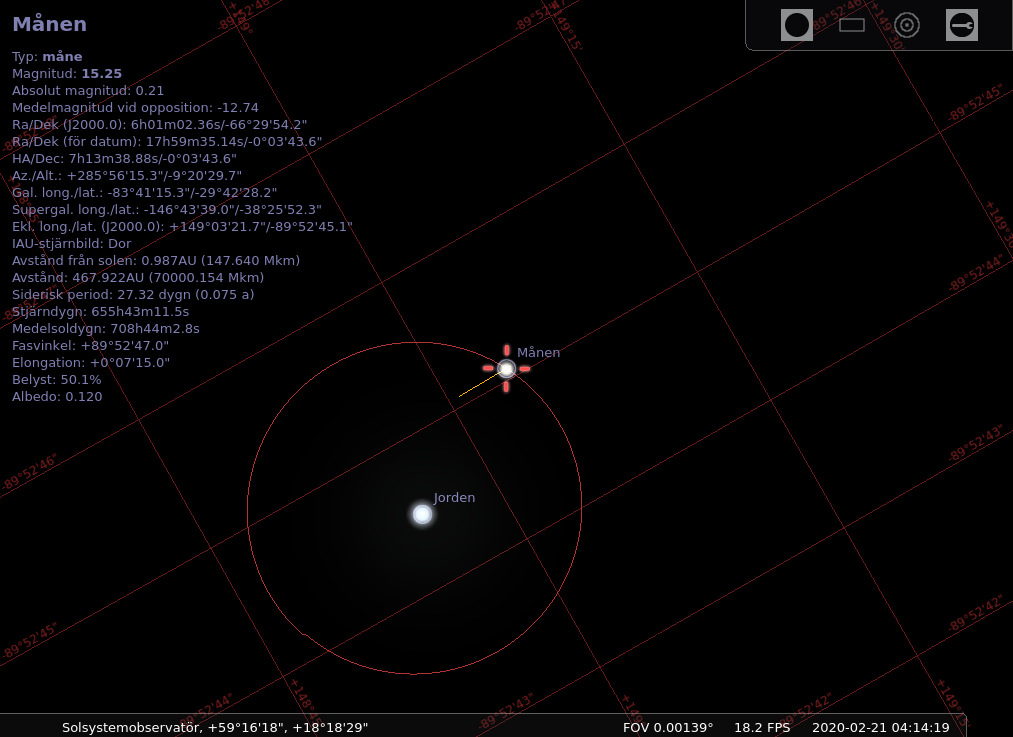
\includegraphics[width=\textwidth]{Stellarium1/WXCresc/stellarium-000.png}
         \caption{SSO, 2020-02-21, kl. 04:14}
         \label{fig:y equals x}
     \end{subfigure}
     \hfill
     \begin{subfigure}[b]{0.45\textwidth}
         \centering
         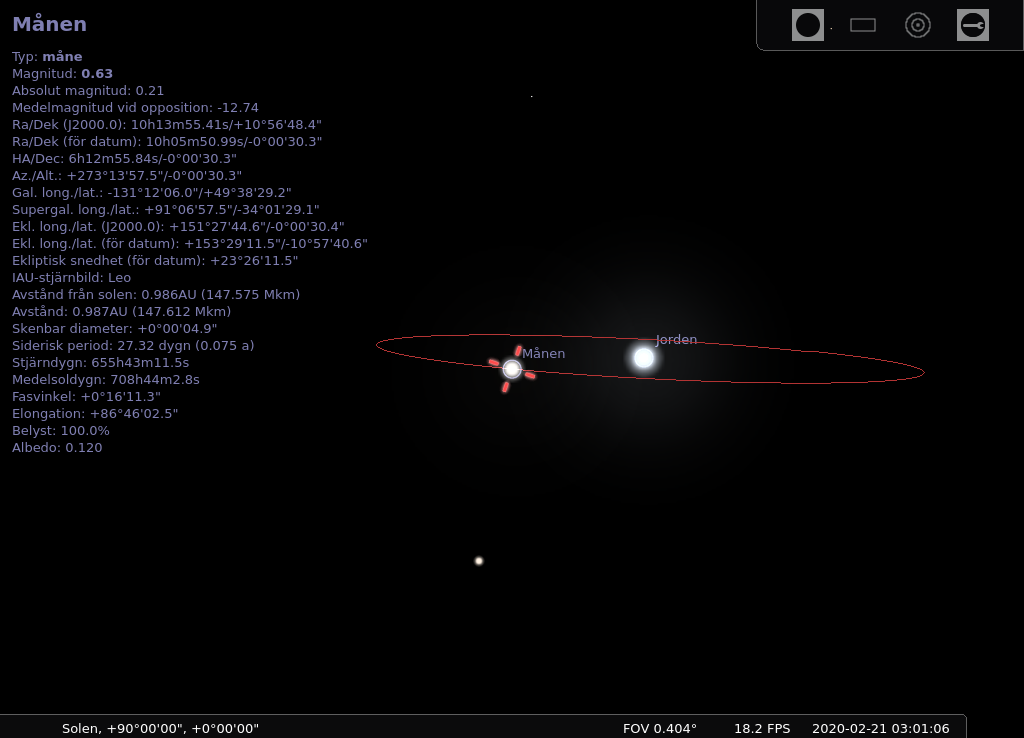
\includegraphics[width=\textwidth]{Stellarium1/WXCresc/stellarium-001.png}
         \caption{Observatör solens nordpol, 2020-02-21, kl. 03:01}
         \label{fig:three sin x}
     \end{subfigure}
     \hfill
     \begin{subfigure}[b]{0.45\textwidth}
         \centering
         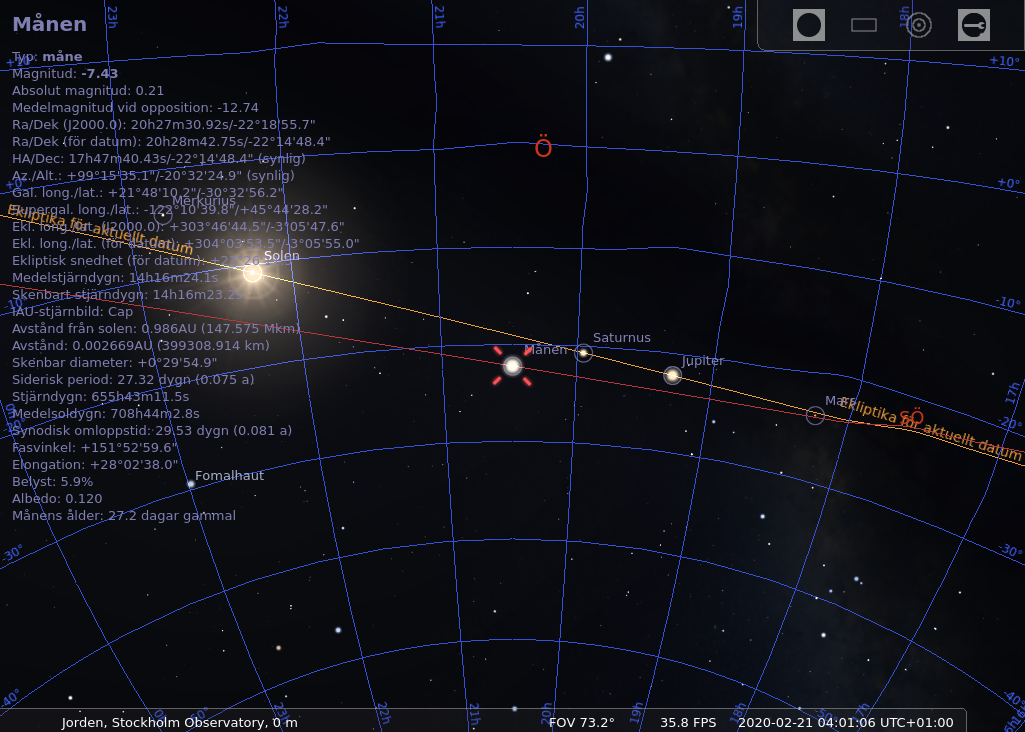
\includegraphics[width=\textwidth]{Stellarium1/WXCresc/stellarium-002.png}
         \caption{Transpararent jord, månen under horisonenten.}
         \label{fig:three sin x}
     \end{subfigure}
     \hfill
     \begin{subfigure}[b]{0.45\textwidth}
         \centering
         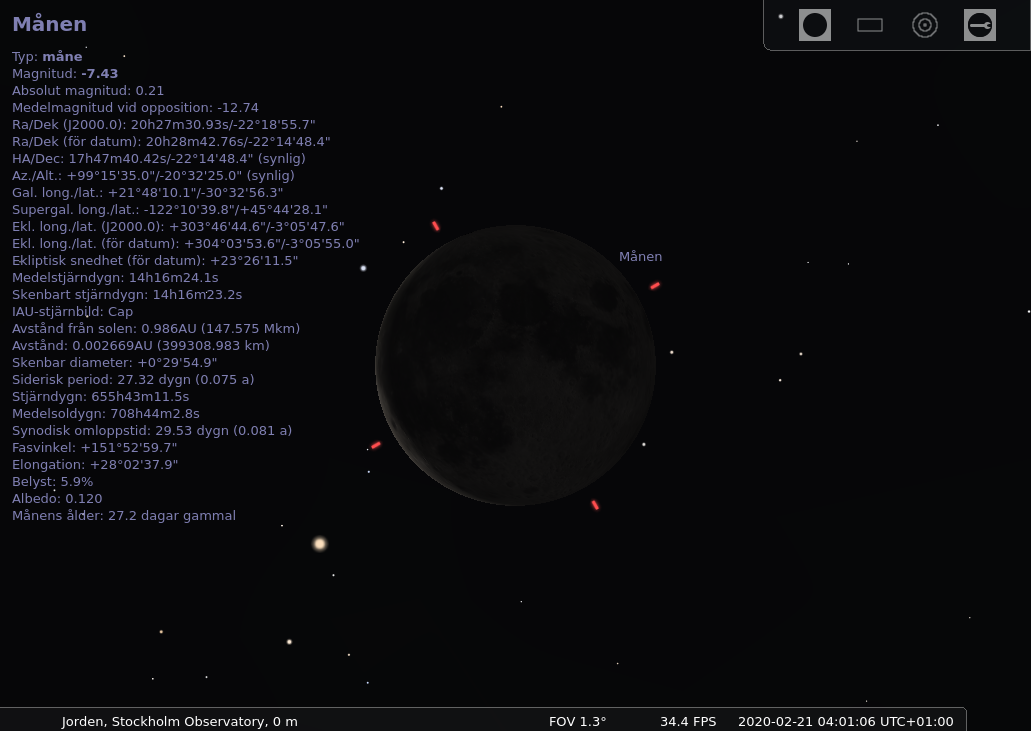
\includegraphics[width=\textwidth]{Stellarium1/WXCresc/stellarium-003.png}
         \caption{Transpararent jord, månen under horisonenten. }
         \label{fig:three sin x}
     \end{subfigure}
     \hfill
        \caption{Waxing crescent }
        \label{fig:perod graphs}
\end{figure}
\newpage
\textit{\textbf{Nymåne enligt Stellariums beräkning}}
\begin{figure}[H]
     \centering
     \begin{subfigure}[b]{0.45\textwidth}
         \centering
         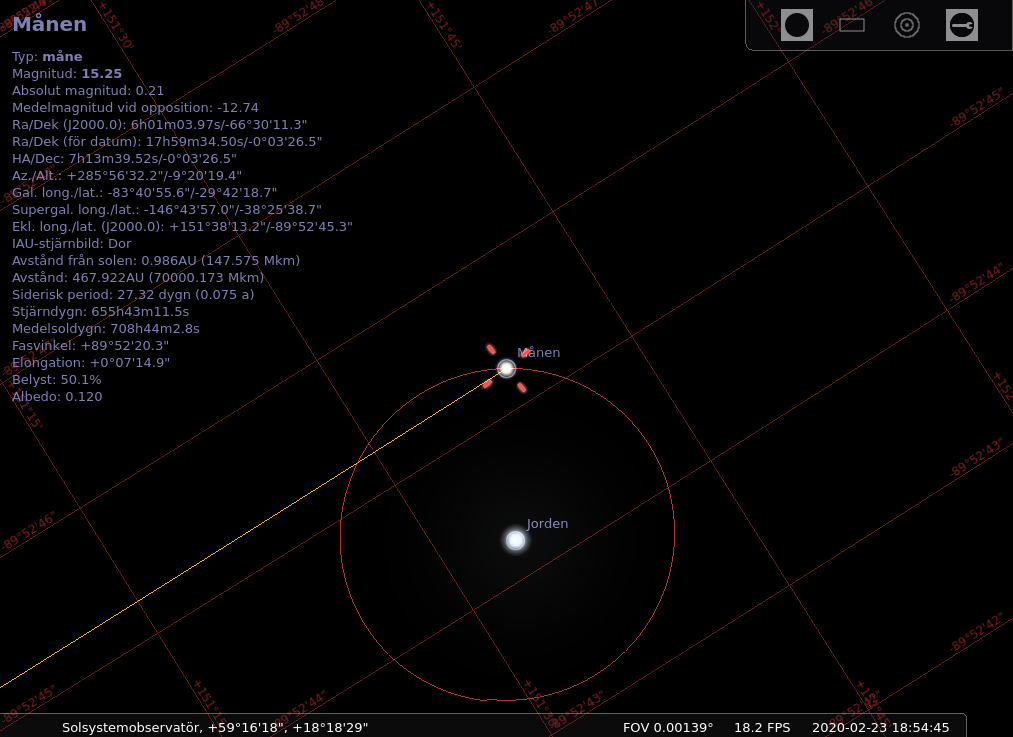
\includegraphics[width=\textwidth]{Stellarium1/NewMoon/stellarium-000.png}
         \caption{SSO, 2020-02-23, kl. 18:54}
         \label{fig:y equals x}
     \end{subfigure}
     \hfill
     \begin{subfigure}[b]{0.45\textwidth}
         \centering
         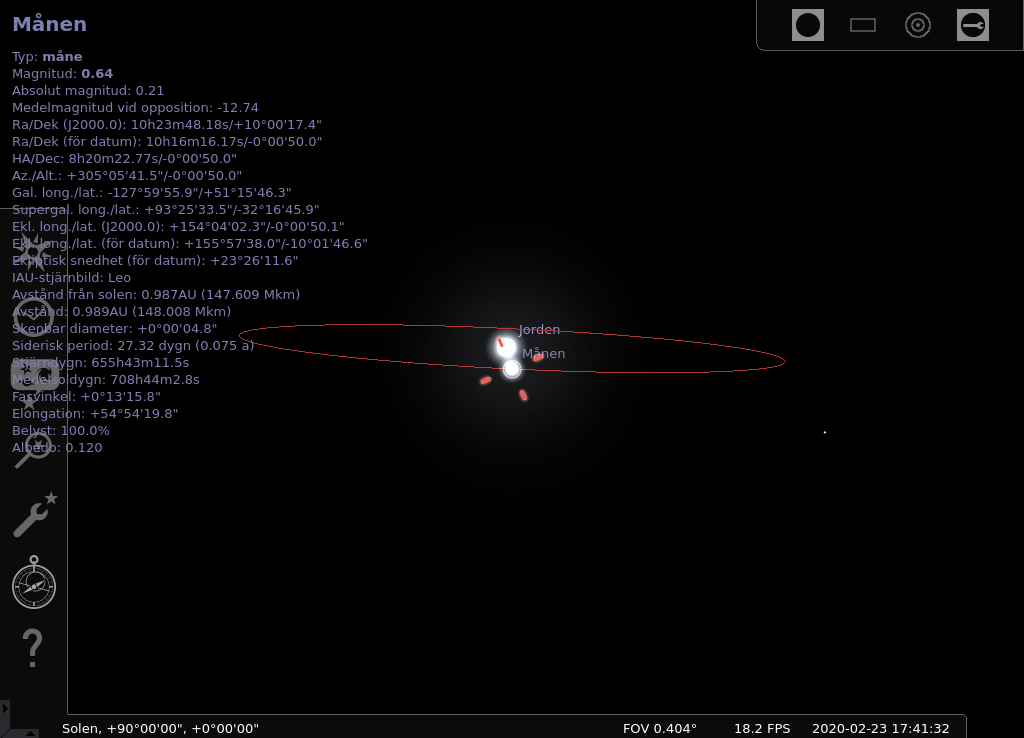
\includegraphics[width=\textwidth]{Stellarium1/NewMoon/stellarium-001.png}
         \caption{Observatör solens nordpol kl. 17:41}
         \label{fig:three sin x}
     \end{subfigure}
     \hfill
     \begin{subfigure}[b]{0.45\textwidth}
         \centering
         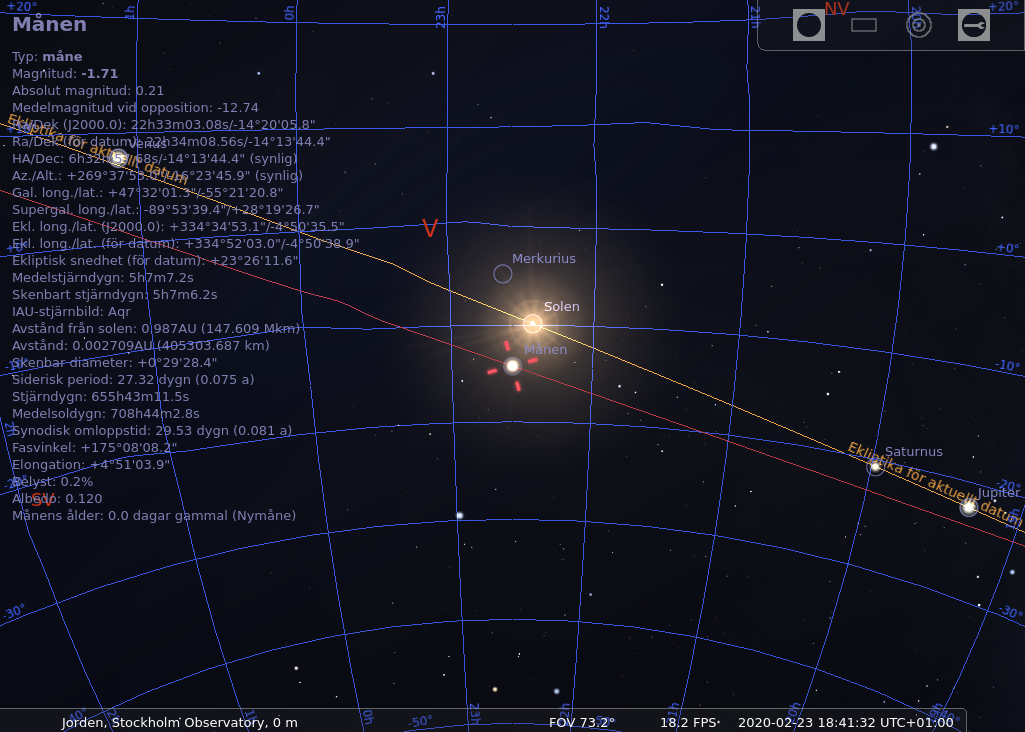
\includegraphics[width=\textwidth]{Stellarium1/NewMoon/stellarium-002.png}
         \caption{Nymåne under horisonten, kl. 18:41}
         \label{fig:three sin x}
     \end{subfigure}
     \hfill
     \begin{subfigure}[b]{0.45\textwidth}
         \centering
         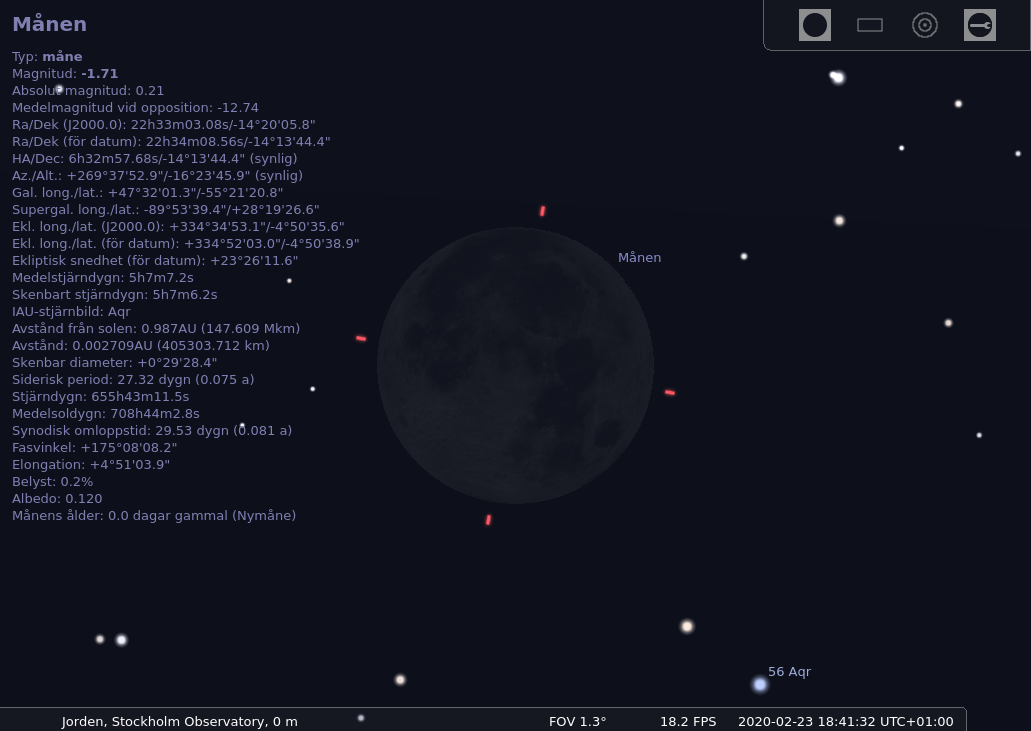
\includegraphics[width=\textwidth]{Stellarium1/NewMoon/stellarium-003.png}
         \caption{Nymåne under horisonten, kl. 18:41}
         \label{fig:three sin x}
     \end{subfigure}
     \hfill
     \begin{subfigure}[b]{0.45\textwidth}
         \centering
         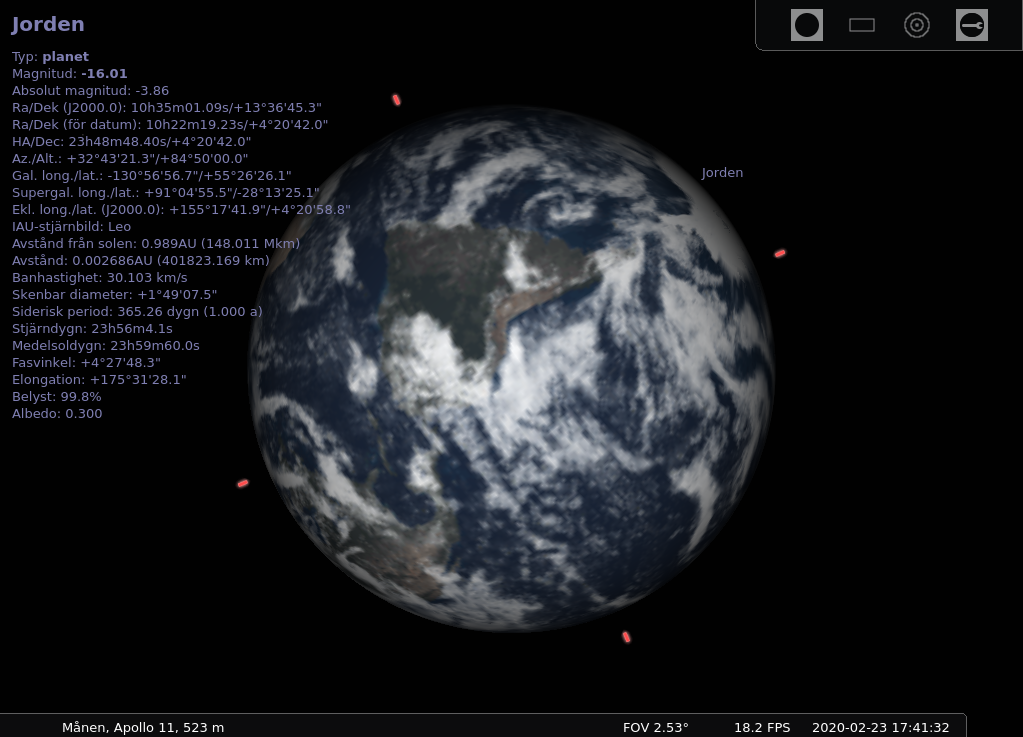
\includegraphics[width=\textwidth]{Stellarium1/NewMoon/stellarium-005.png}
         \caption{Observatör månens nordpol}
         \label{fig:three sin x}
     \end{subfigure}
     \hfill
        \caption{Nymåne enligt Stellariums beräkning }
        \label{fig:perod graphs}
\end{figure}
Diskrepans i tidsynkningen för plugin ``Remote Sync''.
Dålig överensstämmelse mellan SSO och observatör på solens nordpol.
Borde testat hur det ser ut från jordens nordpol.
\newpage
\textit{\textbf{Nymåne enligt Solsystemsobservatör}}
\begin{figure}[H]
     \centering
     \begin{subfigure}[b]{0.45\textwidth}
         \centering
         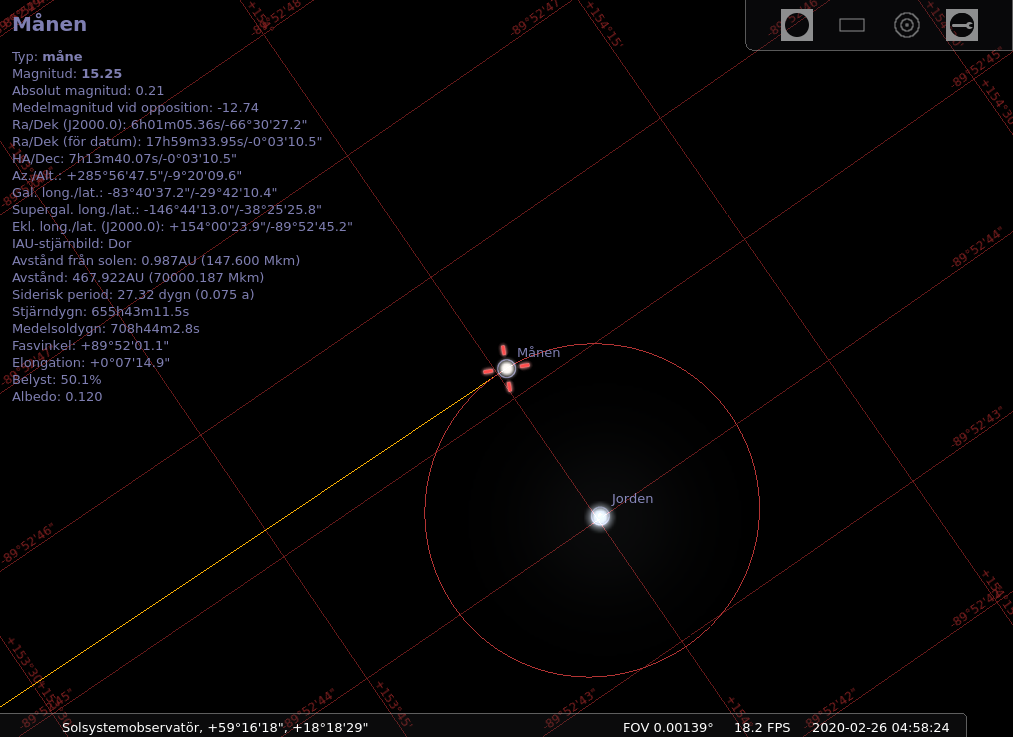
\includegraphics[width=\textwidth]{Stellarium1/RealNewMoon/stellarium-000.png}
         \caption{SSO, 2020-02-26, kl. 04:58}
         \label{fig:y equals x}
     \end{subfigure}
     \hfill
     \begin{subfigure}[b]{0.45\textwidth}
         \centering
         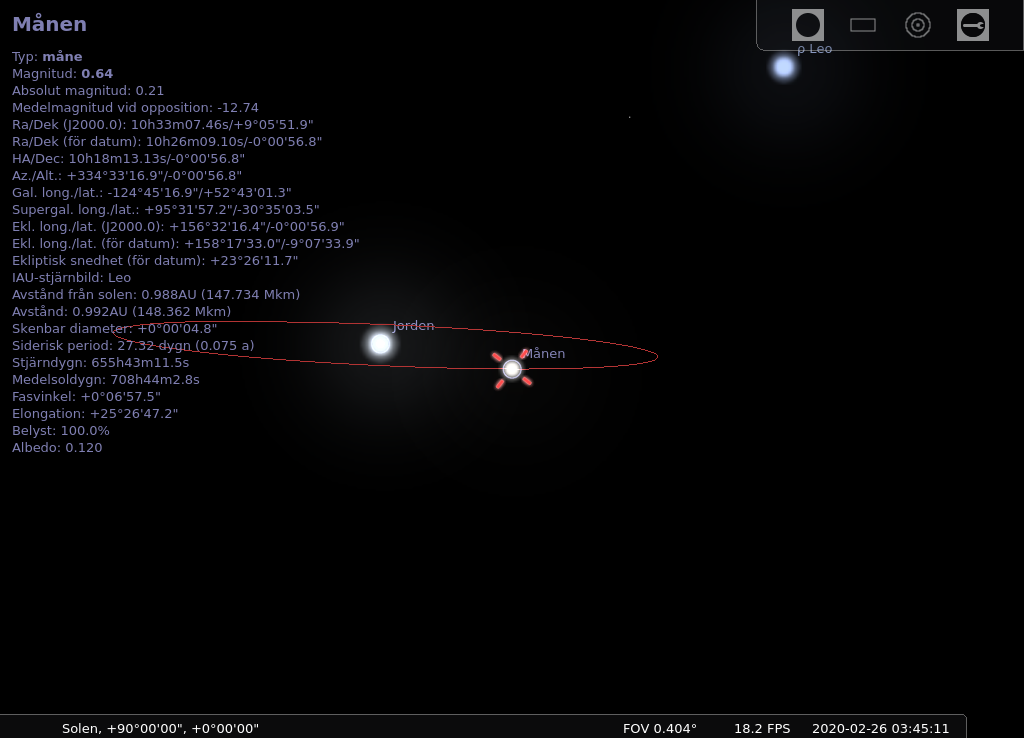
\includegraphics[width=\textwidth]{Stellarium1/RealNewMoon/stellarium-001.png}
         \caption{Observatör solens nordpol, kl. 03:45}
         \label{fig:three sin x}
     \end{subfigure}
     \hfill
     \begin{subfigure}[b]{0.45\textwidth}
         \centering
         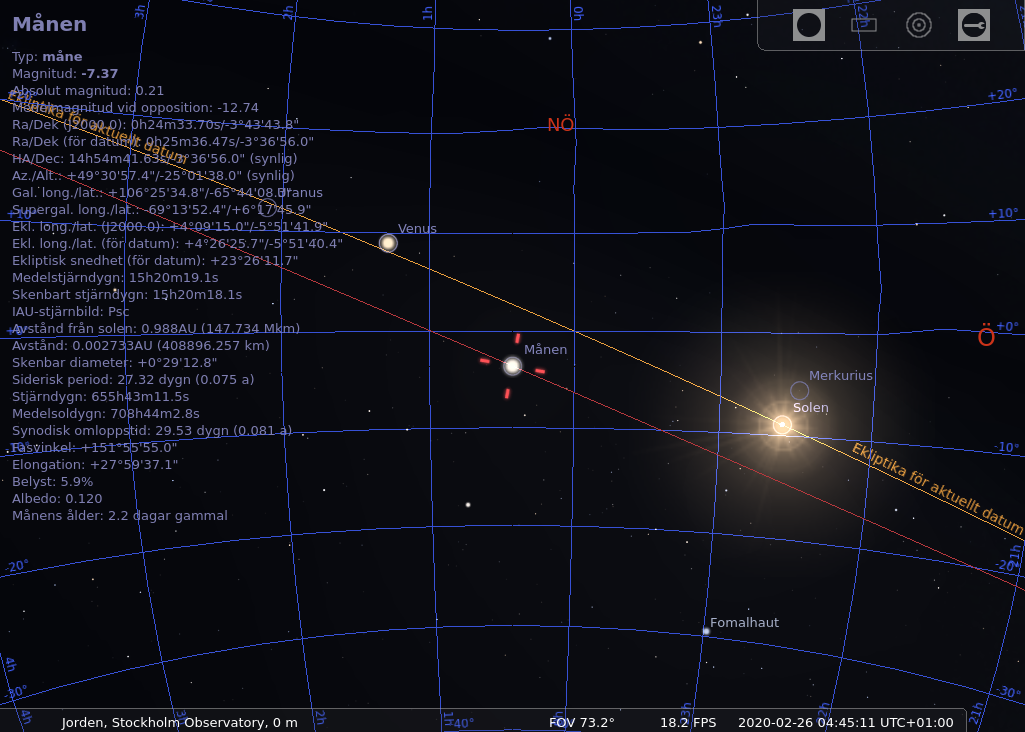
\includegraphics[width=\textwidth]{Stellarium1/RealNewMoon/stellarium-002.png}
         \caption{Månen under horisonten, kl. 04:45}
         \label{fig:three sin x}
     \end{subfigure}
     \hfill
     \begin{subfigure}[b]{0.45\textwidth}
         \centering
         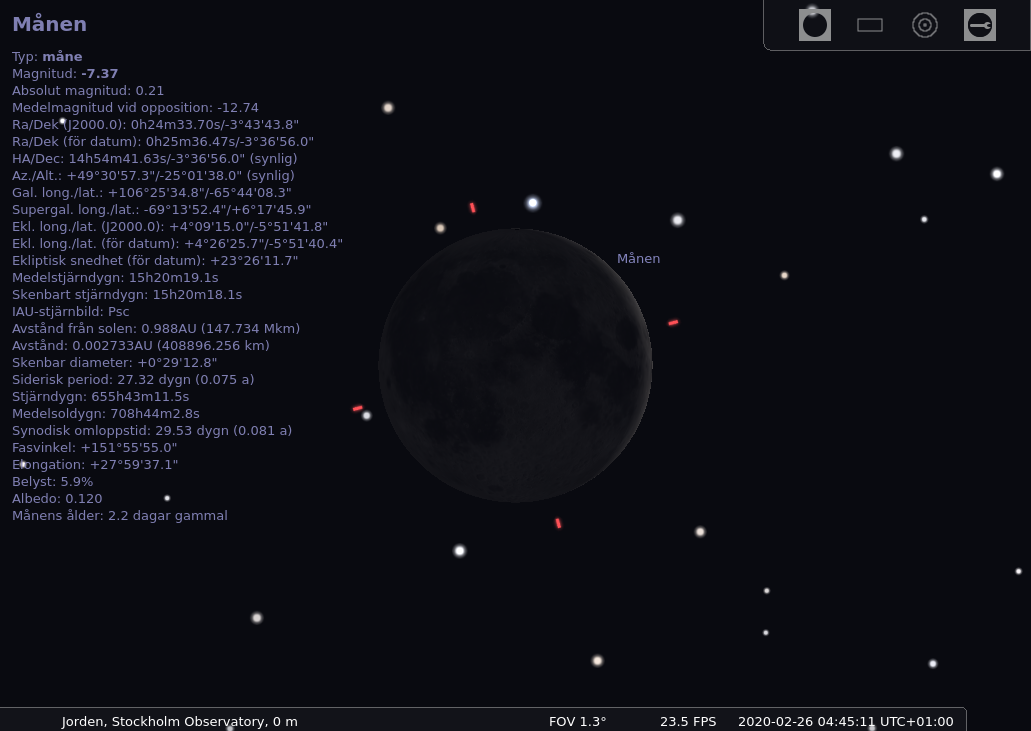
\includegraphics[width=\textwidth]{Stellarium1/RealNewMoon/stellarium-003.png}
         \caption{Månen under horisonten, kl. 04:45}
         \label{fig:three sin x}
     \end{subfigure}
     \hfill
     \begin{subfigure}[b]{0.45\textwidth}
         \centering
         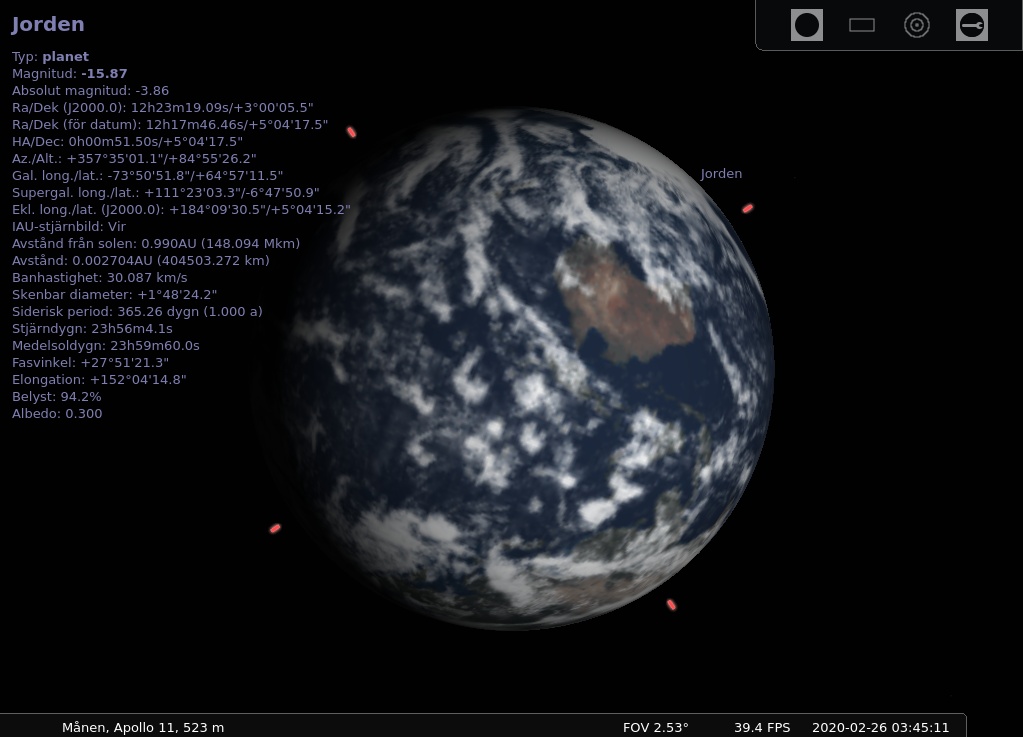
\includegraphics[width=\textwidth]{Stellarium1/RealNewMoon/stellarium-004.png}
         \caption{Observatör månens nordpol}
         \label{fig:three sin x}
     \end{subfigure}
     \hfill
        \caption{Nymåne för Solsystemsobservatör }
        \label{fig:perod graphs}
\end{figure}
Koordinaterna för observatören på månens nordpol överensstämmer
inte med texten ``Apollo 11''. Diskrepans i tidsynkningen
för plugin ``Remote Sync''.
\newpage
\textit{\textbf{Waning Crescent måne}}
\begin{figure}[H]
     \centering
     \begin{subfigure}[b]{0.45\textwidth}
         \centering
         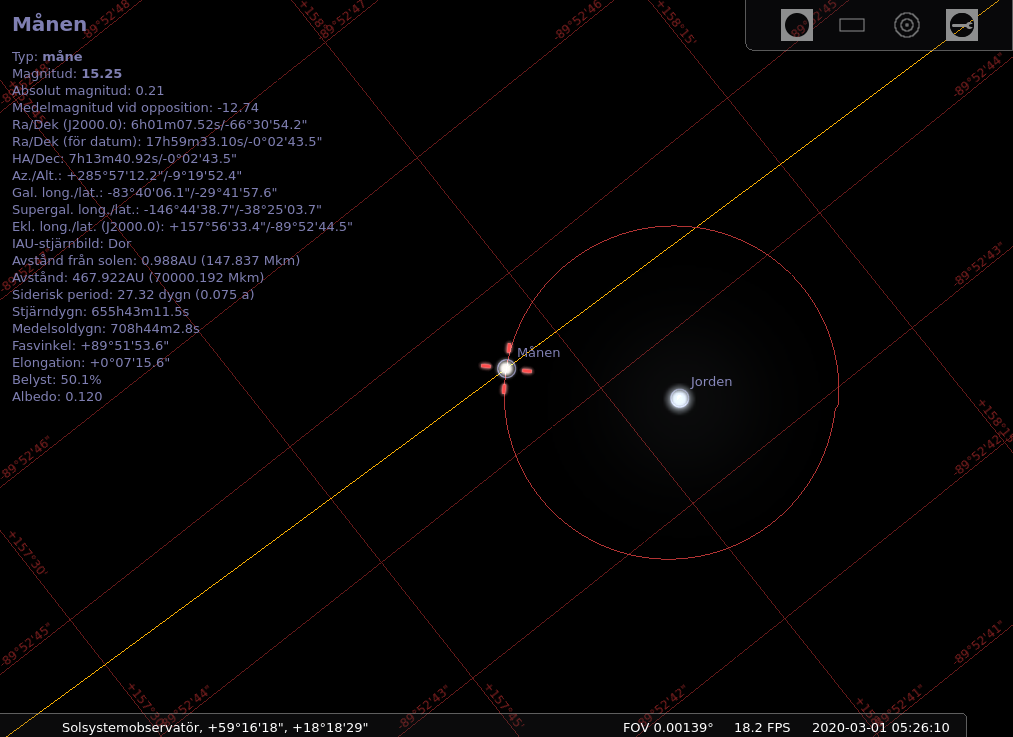
\includegraphics[width=\textwidth]{Stellarium1/WaningCrescent/stellarium-000.png}
         \caption{SSO, 2020-03-01, kl. 05:26}
         \label{fig:y equals x}
     \end{subfigure}
     \hfill
     \begin{subfigure}[b]{0.45\textwidth}
         \centering
         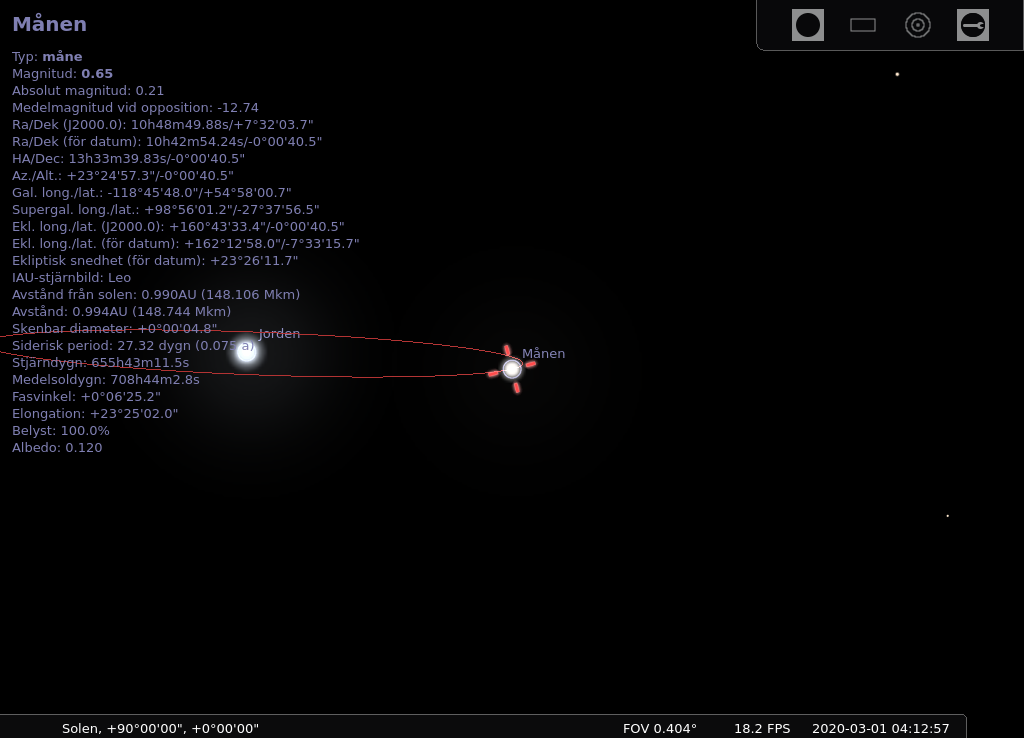
\includegraphics[width=\textwidth]{Stellarium1/WaningCrescent/stellarium-001.png}
         \caption{Observator solnordpol. Månen till höger om jorden.}
         \label{fig:three sin x}
     \end{subfigure}
     \hfill
     \begin{subfigure}[b]{0.45\textwidth}
         \centering
         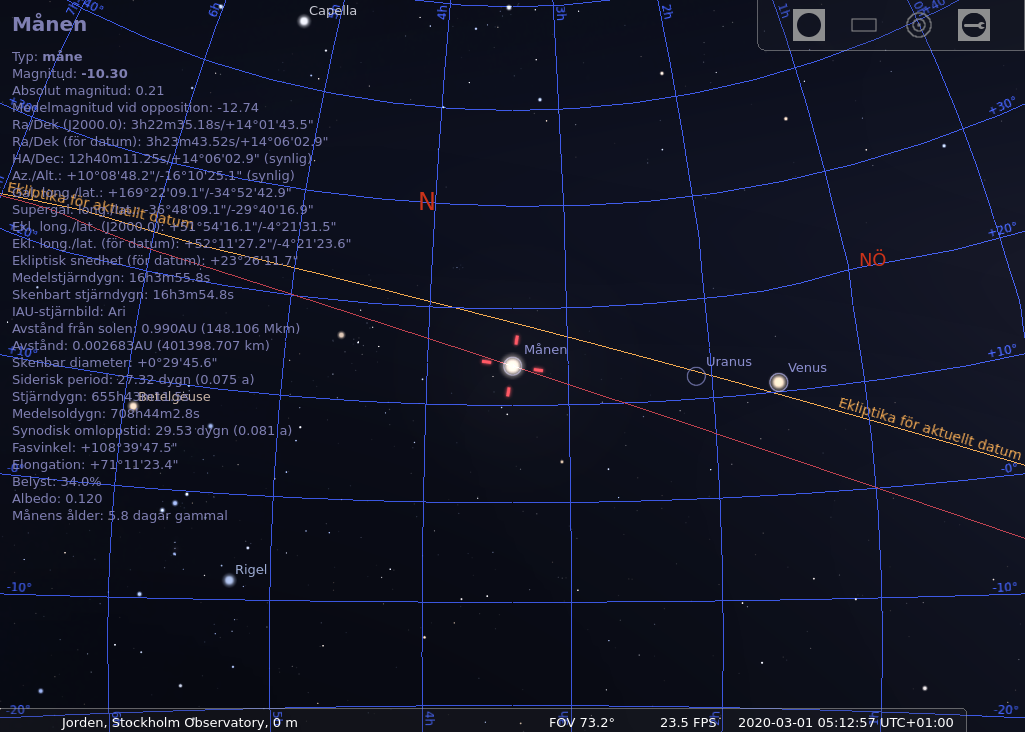
\includegraphics[width=\textwidth]{Stellarium1/WaningCrescent/stellarium-002.png}
         \caption{Måne över horistonten}
         \label{fig:three sin x}
     \end{subfigure}
     \hfill
     \begin{subfigure}[b]{0.45\textwidth}
         \centering
         \includegraphics[width=\textwidth]{Stellarium1/WaningCrescent/stellarium-003.png}
         \caption{Måne över horistonten}
         \label{fig:three sin x}
     \end{subfigure}
     \hfill
     \begin{subfigure}[b]{0.45\textwidth}
         \centering
         \includegraphics[width=\textwidth]{Stellarium1/WaningCrescent/stellarium-004.png}
         \caption{Observatör på månens nordpol}
         \label{fig:three sin x}
     \end{subfigure}
     \hfill
        \caption{ Waning Crescent måne}
        \label{fig:perod graphs}
\end{figure}
Månobservatörens vy verkar inte vara korrekt, det ser ut som att man
ser Australien från månen. Stockholm ligger på diametralt
motsatt sida ungerfär.$+10^\circ$ innebär att månen är synlig ovanför
horsionten från Stockholm, korrekt?
\newpage
\textit{\textbf{Första kvarten}}
\begin{figure}[H]
     \centering
     \begin{subfigure}[b]{0.45\textwidth}
         \centering
         \includegraphics[width=\textwidth]{Stellarium1/FirstQuarter/stellarium-000.png}
         \caption{SSO, 2020-03-05, kl. 09:16}
         \label{fig:y equals x}
     \end{subfigure}
     \hfill
     \begin{subfigure}[b]{0.45\textwidth}
         \centering
         \includegraphics[width=\textwidth]{Stellarium1/FirstQuarter/stellarium-001.png}
         \caption{Solnordpols Observatör kl. 07:47}
         \label{fig:three sin x}
     \end{subfigure}
     \hfill
     \begin{subfigure}[b]{0.45\textwidth}
         \centering
         \includegraphics[width=\textwidth]{Stellarium1/FirstQuarter/stellarium-002.png}
         \caption{Stockholm, kl. 08:47}
         \label{fig:three sin x}
     \end{subfigure}
     \hfill
     \begin{subfigure}[b]{0.45\textwidth}
         \centering
         \includegraphics[width=\textwidth]{Stellarium1/FirstQuarter/stellarium-003.png}
         \caption{Stockholm, kl. 08:47}
         \label{fig:three sin x}
     \end{subfigure}
     \hfill
     \begin{subfigure}[b]{0.45\textwidth}
         \centering
         \includegraphics[width=\textwidth]{Stellarium1/FirstQuarter/stellarium-004.png}
         \caption{Månnordpolsobservatör}
         \label{fig:three sin x}
     \end{subfigure}
     \hfill
        \caption{ Första kvarten }
        \label{fig:perod graphs}
\end{figure}
Skuggan på jorden bör vara lodrät sedd från månens nordpol
\newpage
\textit{\textbf{Waning Gibbons måne}}
\begin{figure}[H]
     \centering
     \begin{subfigure}[b]{0.45\textwidth}
         \centering
         \includegraphics[width=\textwidth]{Stellarium1/WaningGibbons/stellarium-005.png}
         \caption{SSO, 2020-03-08, kl. 13:34}
         \label{fig:y equals x}
     \end{subfigure}
     \hfill
     \begin{subfigure}[b]{0.45\textwidth}
         \centering
         \includegraphics[width=\textwidth]{Stellarium1/WaningGibbons/stellarium-006.png}
         \caption{Solnordpolsobservatör, kl. 12:22}
         \label{fig:three sin x}
     \end{subfigure}
     \hfill
     \begin{subfigure}[b]{0.45\textwidth}
         \centering
         \includegraphics[width=\textwidth]{Stellarium1/WaningGibbons/stellarium-007.png}
         \caption{Stockholmsobservatör, kl. 13:22}
         \label{fig:three sin x}
     \end{subfigure}
     \hfill
     \begin{subfigure}[b]{0.45\textwidth}
         \centering
         \includegraphics[width=\textwidth]{Stellarium1/WaningGibbons/stellarium-008.png}
         \caption{Stockholmsobservatör, kl. 13:22}
         \label{fig:three sin x}
     \end{subfigure}
     \hfill
     \begin{subfigure}[b]{0.45\textwidth}
         \centering
         \includegraphics[width=\textwidth]{Stellarium1/WaningGibbons/stellarium-009.png}
         \caption{Månnordpolsobeservatör}
         \label{fig:three sin x}
     \end{subfigure}
     \hfill
        \caption{ Waning gibbons}
        \label{fig:perod graphs}
\end{figure}
Jorden bör ha en elliptisk skugga istället för en rund skugg sedd från 
månens nordpol.
\newpage
\textit{\textbf{Fullmåne enligt Solsystemsobservatören}}
\begin{figure}[H]
     \centering
     \begin{subfigure}[b]{0.45\textwidth}
         \centering
         \includegraphics[width=\textwidth]{Stellarium1/SSONewMoon/stellarium-000.png}
         \caption{SSO, 2020-03-12, kl. 09:39}
         \label{fig:y equals x}
     \end{subfigure}
     \hfill
     \begin{subfigure}[b]{0.45\textwidth}
         \centering
         \includegraphics[width=\textwidth]{Stellarium1/SSONewMoon/stellarium-001.png}
         \caption{Solnordpolsobservatör, kl. 08:26}
         \label{fig:three sin x}
     \end{subfigure}
     \hfill
     \begin{subfigure}[b]{0.45\textwidth}
         \centering
         \includegraphics[width=\textwidth]{Stellarium1/SSONewMoon/stellarium-002.png}
         \caption{Måne under horisonten, kl.09:26}
         \label{fig:three sin x}
     \end{subfigure}
     \hfill
     \begin{subfigure}[b]{0.45\textwidth}
         \centering
         \includegraphics[width=\textwidth]{Stellarium1/SSONewMoon/stellarium-003.png}
         \caption{Måne under horisonten, kl.09:26}
         \label{fig:three sin x}
     \end{subfigure}
     \hfill
     \begin{subfigure}[b]{0.45\textwidth}
         \centering
         \includegraphics[width=\textwidth]{Stellarium1/FirstQuarter/stellarium-004.png}
         \caption{Månnordpolsobservatör, kl. 07:47}
         \label{fig:three sin x}
     \end{subfigure}
     \hfill
        \caption{ Fullmåne enligt inspektionenligt SSO}
        \label{fig:perod graphs}
\end{figure}
Månnordpols observatören bör se en helt svart skiv, tror jag, därför att
 måncentrum befinner sig på ca -10 grader enligt figure c vilket borde
betyda att siktlinjen för månobservatören är ungefär på jordens ekvator.

\newpage
\item[--] Hur ligger månens bana i förhållande till ekliptikan?\\

Månens bana korsar eklipitikan vid första kvarten och tredje kvarten, se bild
nedan\footnote{\url{https://en.wikipedia.org/wiki/Orbit_of_the_Moon\#/media/File:Lunar_perturbation.jpg}}.
Under ekliptikan efter första varten till fullmånen till tredje kvarten och från tredje
kvarten ovanför ekliptikan.
\begin{figure}[H]
\centering
  \includegraphics[scale=0.4]{Lunar_perturbation.jpg}
  \caption{Månens rörelse i förhållande till ekliptikan }
  \label{fig4}
\end{figure}
\item[--] Genom att välja Solsystemsobservatör igen och zooma in på jorden kan du få en överblick
över jorden och månen. Låt tiden gå. Kan du se hur månen belyses av solen och hur detta
kan ses från jorden? \\

Delvis svårt emellanåt p.g.a. att Stellarium inte verkar beräkna skuggprojektionen
utan verkar använda fotografier. Se bildkollage ovan.
Vidare så minskas förtroendet p.g.a. att tidssynkning inte fungerar
mellan solsystems observatören och andra observatörer.
\newpage
\item[--] Den 27 juli 2018 kunde man se en vacker månförmörkelse.
 Hur ser den ut i programmet?\\
 
 Det verkar som att månen blivit mörk p.g.a. att observatören
blivit bländand av reflekterat ljud från Mars, kan det stämma?
\begin{figure}[H]
     \centering
     \begin{subfigure}[b]{0.45\textwidth}
         \centering
         \includegraphics[width=\textwidth]{Stellarium1/20180727/stellarium-000.png}
         \caption{}
         \label{fig:y equals x}
     \end{subfigure}
     \hfill
     \begin{subfigure}[b]{0.45\textwidth}
         \centering
         \includegraphics[width=\textwidth]{Stellarium1/20180727/stellarium-001.png}
         \caption{}
         \label{fig:three sin x}
     \end{subfigure}
     \hfill
     \begin{subfigure}[b]{0.45\textwidth}
         \centering
         \includegraphics[width=\textwidth]{Stellarium1/20180727/stellarium-002.png}
         \caption{}
         \label{fig:three sin x}
     \end{subfigure}
     \hfill
     \begin{subfigure}[b]{0.45\textwidth}
         \centering
         \includegraphics[width=\textwidth]{Stellarium1/20180727/stellarium-003.png}
         \caption{}
         \label{fig:three sin x}
     \end{subfigure}
     \hfill
        \caption{ Fullmåne 2018-07-27 blir förmörkad}
        \label{fig:perod graphs}
\end{figure}
\end{itemize}
\newpage
\section{Solens årliga rörelse över himlen}
\begin{itemize}
\item[--] Hur ändras solens höjd och vilken figur beskriver den under loppet av ett år?\\

Solens läge på himlen kallas ``analemma'' mätt vid fix tidpunkt varje dagbeskriver en figur som liknar siffran 8, 
se\footnote{\url{https://sv.wikipedia.org/wiki/Analemma\#/media/Fil:Analemma_pattern_in_the_sky.jpg}}
\begin{figure}[H]
\centering
  \includegraphics[scale=0.4]{Analemma_pattern_in_the_sky.jpeg}
  \caption{Analemma - solens rörelse vid fixa tidpunkter över året}
  \label{fig4}
\end{figure}
 
\item[--]Varför? \\

Personligen anser jag det vara svårt att visualisera varför analemma-figuren blir som den blir men
naturligtvis beror detta på ekliptikans lutning och jordbanans eccentricitet.
Man kan se detta i Stellarium om man avancererar tiden genom att stega tiden en vecka i taget med \verb+]+
\end{itemize}
\newpage
\section{Resa i tid och rum}
\begin{itemize}
\item[--] Gör avslutningsvis en liten resa i universum. Du bör nu ha rätt bra koll på ’kontrollerna‘ så att du
kan röra dig ganska fritt.
Zooma in dig på olika spännade objekt från t ex Messier-katalogen, besök olika stjärnor och svep
genom universum! Upplev möjligheterna med detta program!\\

Messier-katalogen är förvisso intressant men då önskan är att lära sig parallax-mätning av avstånd
exempelvistill $\alpha$-Centauri så irriterar arbetsuppgiften snarare är skänker stimulans.
Önskar lära mig mäta parallax mäta i Stellarium men stöter på patrull och vet inte hur jag ska göra
\begin{figure}[H]
     \centering
     \begin{subfigure}[b]{0.45\textwidth}
         \centering
         \includegraphics[width=\textwidth]{Stellarium1/Centauri/stellarium-001.png}
         \caption{}
         \label{fig:y equals x}
     \end{subfigure}
     \hfill
     \begin{subfigure}[b]{0.45\textwidth}
         \centering
         \includegraphics[width=\textwidth]{Stellarium1/Centauri/stellarium-002.png}
         \caption{}
         \label{fig:three sin x}
     \end{subfigure}
     \hfill
     \begin{subfigure}[b]{0.45\textwidth}
         \centering
         \includegraphics[width=\textwidth]{Stellarium1/Centauri/stellarium-004.png}
         \caption{}
         \label{fig:three sin x}
     \end{subfigure}
     \hfill
     \begin{subfigure}[b]{0.45\textwidth}
         \centering
         \includegraphics[width=\textwidth]{Stellarium1/Centauri/stellarium-005.png}
         \caption{}
         \label{fig:three sin x}
     \end{subfigure}
     \hfill
        \caption{ Misslyckat försök att mäta avstånd till $\alpha$ Centauri }
        \label{fig:perod graphs}
\end{figure}
Mätt att grannstjärnan rört sig ca 60 grader. Jordens banradie är 6371.2 km
men hur kompenserar jag för det faktum att teleskopet har zoomat in och vinkeln förstorats?
Behöver en förstoringsfaktor $k$.Hur fås denna fram?
\begin{flalign*}
k\cdot tan(30^\circ)&=\frac{6371.2}{h}\iff\\
h            &=\frac{6371.2}{k\cdot tan(30^\circ)}
\end{flalign*}


\end{itemize}
%\underbrace{}

% \hspace{1em}

%\begin{enumerate}[label=(\alph*)]
%\end{enumerate}

%$$
%  A = 
%  \begin{bmatrix}
%    1 & 0  & 2i\\
%    2i & 0 &  -4\\
%    -i &  0 & -2i\\
%  \end{bmatrix}
%$$

%\begin{flalign*}
%  A = 
%  \begin{bmatrix}
%    1 & 0  & 2i\\
%    2i & 0 &  -4\\
%    -i &  0 & -2i\\
%  \end{bmatrix}
%\end{flalign*}


%\begin{flalign*}
%\psi(x) = \begin{cases} Ae^{ikx}+Be^{-ikx} &\ \  x<-a \\
%                        Ce^{\kappa x}+De^{-\kappa x} &\ \ -a < x < a\\
%						Fe^{ikx} & \ \ x>a
%       \end{cases}
%\end{flalign*}
%[width=80mm,scale=0.7]
%\begin{figure}[H]
\centering
%  \includegraphics[width=\linewidth]{odd_finite.eps}
%  \caption{$z_0=0.1\pi,0.5\pi, 3\pi,7\pi$}
%  \label{fig4}
%\end{figure}
\end{document}

\begin{figure}[htbp]
     \centering
     \begin{subfigure}[b]{0.45\textwidth}
         \centering
         \includegraphics[width=\textwidth]{Stellarium/}
         \caption{SSO utzoomad 2020-02-13, kl. 17:50}
         \label{fig:y equals x}
     \end{subfigure}
     \hfill
     \begin{subfigure}[b]{0.45\textwidth}
         \centering
         \includegraphics[width=\textwidth]{Stellarium/}
         \caption{SSO 2020-02-13, kl. 17:50}
         \label{fig:three sin x}
     \end{subfigure}
     \hfill
     \begin{subfigure}[b]{0.45\textwidth}
         \centering
         \includegraphics[width=\textwidth]{Stellarium/}
         \caption{SSO 2020-02-13, kl. 17:50}
         \label{fig:three sin x}
     \end{subfigure}
     \hfill
        \caption{ }
        \label{fig:perod graphs}
\end{figure}










                                     
                                     



